\chapter{Surface Event Pulse Shape Simulations}

\section{Introduction}

The events on passivated surfaces create a unique modeling challenge in HPGe detectors. These interactions can be best understood with alphas since they deposit energy over short distances on the surface, creating large charge clouds with complex drift and collection processes. We thus study the events in terms of alpha, but the same can be applied to other passivated surface backgrounds such as $\beta$. This chapter begins by reviewing alpha backgrounds, then discusses the challenges in modeling surface backgrounds and introduces a new model to address these challenges.



\section{Surface Alphas}
\label{ch3_sec_alpha}
\subsection{Properties of Alpha Interactions}
Alpha particles are composed of two protons and two neutrons tightly bound together. They are identical to ionized Helium ions but carry a charge of $+2$ e. The energy of alpha particles is correlated with the half-life of the parent isotope, such that the ones with the highest energies are from parent atoms with the shortest half-lives. Thus, the energies of alpha particles are normally between about $4$ and $6$ MeV. For a given material, the linear stopping power S is defined as $-\frac{dE}{dx}$. The energy loss of charged particles in a material is then given by the Bethe formula:

\begin{equation}\label{bethe_formula}
    -\frac{dE}{dx} = \frac{4\pi e^4z^2}{m_0\nu^2}NB
\end{equation}

such that

\begin{equation}\label{bethe_B}
    \text{B}=Z\left[ \text{ln}\frac{2m_0\nu^2}{I}-\text{ln}\right(1-\frac{\nu^2}{c^2}\left)-\frac{\nu^2}{c^2}\right]
\end{equation}

Here $\nu$ and $ze$ are the charges of the given particle, N and Z are the number density and the atomic number of the absorber atoms, and  m$_0$ and e are the rest mass and charge of the electron, respectively. Parameter I represents the average excitation and ionization potential of the absorber and is normally determined experimentally. 

Eq. \ref{bethe_formula} suggests that the energy loss for non-relativistic particles is proportional to $1/\nu^2$, or the kinetic energy. Hence, the slower the velocity, the longer the particles spend in the vicinity of electrons of the material's atoms, and the higher the energy loss. Eq. \ref{bethe_formula} is proportional to z$^2$ for constant velocity. Thus, the heavier particles will have more energy loss for a given velocity. This results in alphas having a very low penetration depth, usually around $10$ micrometers.

Energy loss of alpha particles can be best understood by plotting specific energy loss along the track. The plot known as the Bragg curve is shown in Fig. \ref{bragg_curve_fig}. During most of the track, the energy loss increases roughly as 1/E as predicted by Eq.\ref{bethe_formula}. As the particles slow down, electron pickup reduces the charge and the curve falls off. As a result, alpha deposits a large amount of energy in a very localized area. For Germanium, this penetration depth of alpha particles is about $17.6$ - $20.0$ microns \cite{knoll_2010}. The n+ electrode and p+ electrode in LEGEND detectors are too thick for alphas to penetrate and deposit much energy. Therefore, alpha events mostly appear only on the passivated surface.

\begin{figure}
\centering
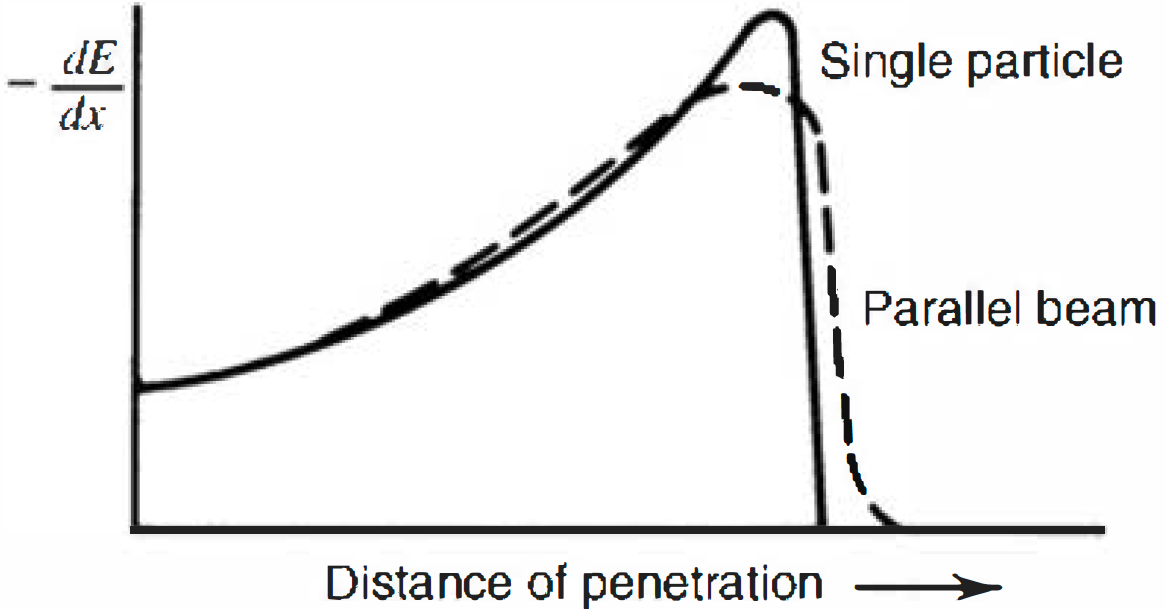
\includegraphics[width=0.5\linewidth]{ch3/figs/bragg_curve.png}
\caption{The specific energy loss in a material for an alpha particle with several MeV initial energy. Plots are shown for a single alpha particle track and for the average behavior of a parallel beam of alpha particles. Alphas loss most of their energies in a small region. Picture from \cite{knoll_2010}}. 
\label{bragg_curve_fig}
\end{figure}

\section{Challenges in modeling surface events}
An alpha particle deposits energy of about $4$ - $6$ MeV with a penetration depth of about $17.6$ - $20.0$ microns on the passivated surface. This excites a lot of charge carriers and produces a dense charge cloud. In such cases, effects such as diffusion of the charges and self-repulsion among charges become significant. These effects could also push the charge onto the passivated surface. It is known from data that charges on the passivated surface move at slower speeds than in the bulk. This is possibly due to different material properties, weaker electric field, and higher charge trapping \cite{MULLOWNEY201233}. Fig. \ref{fig:dcr_waveform} shows a known alpha waveform in experimental data. The alpha waveform being close to the surface has a much sharper rise than the bulk waveform. However, the tail of the alpha waveform has an upward slope towards the end. This is possible due to late collections of charges on the passivated surface. We call this effect Delayed Charge Recovery Effect \cite{Gruszko:2017kfx}.

  \begin{figure}[!htb]
\centering
  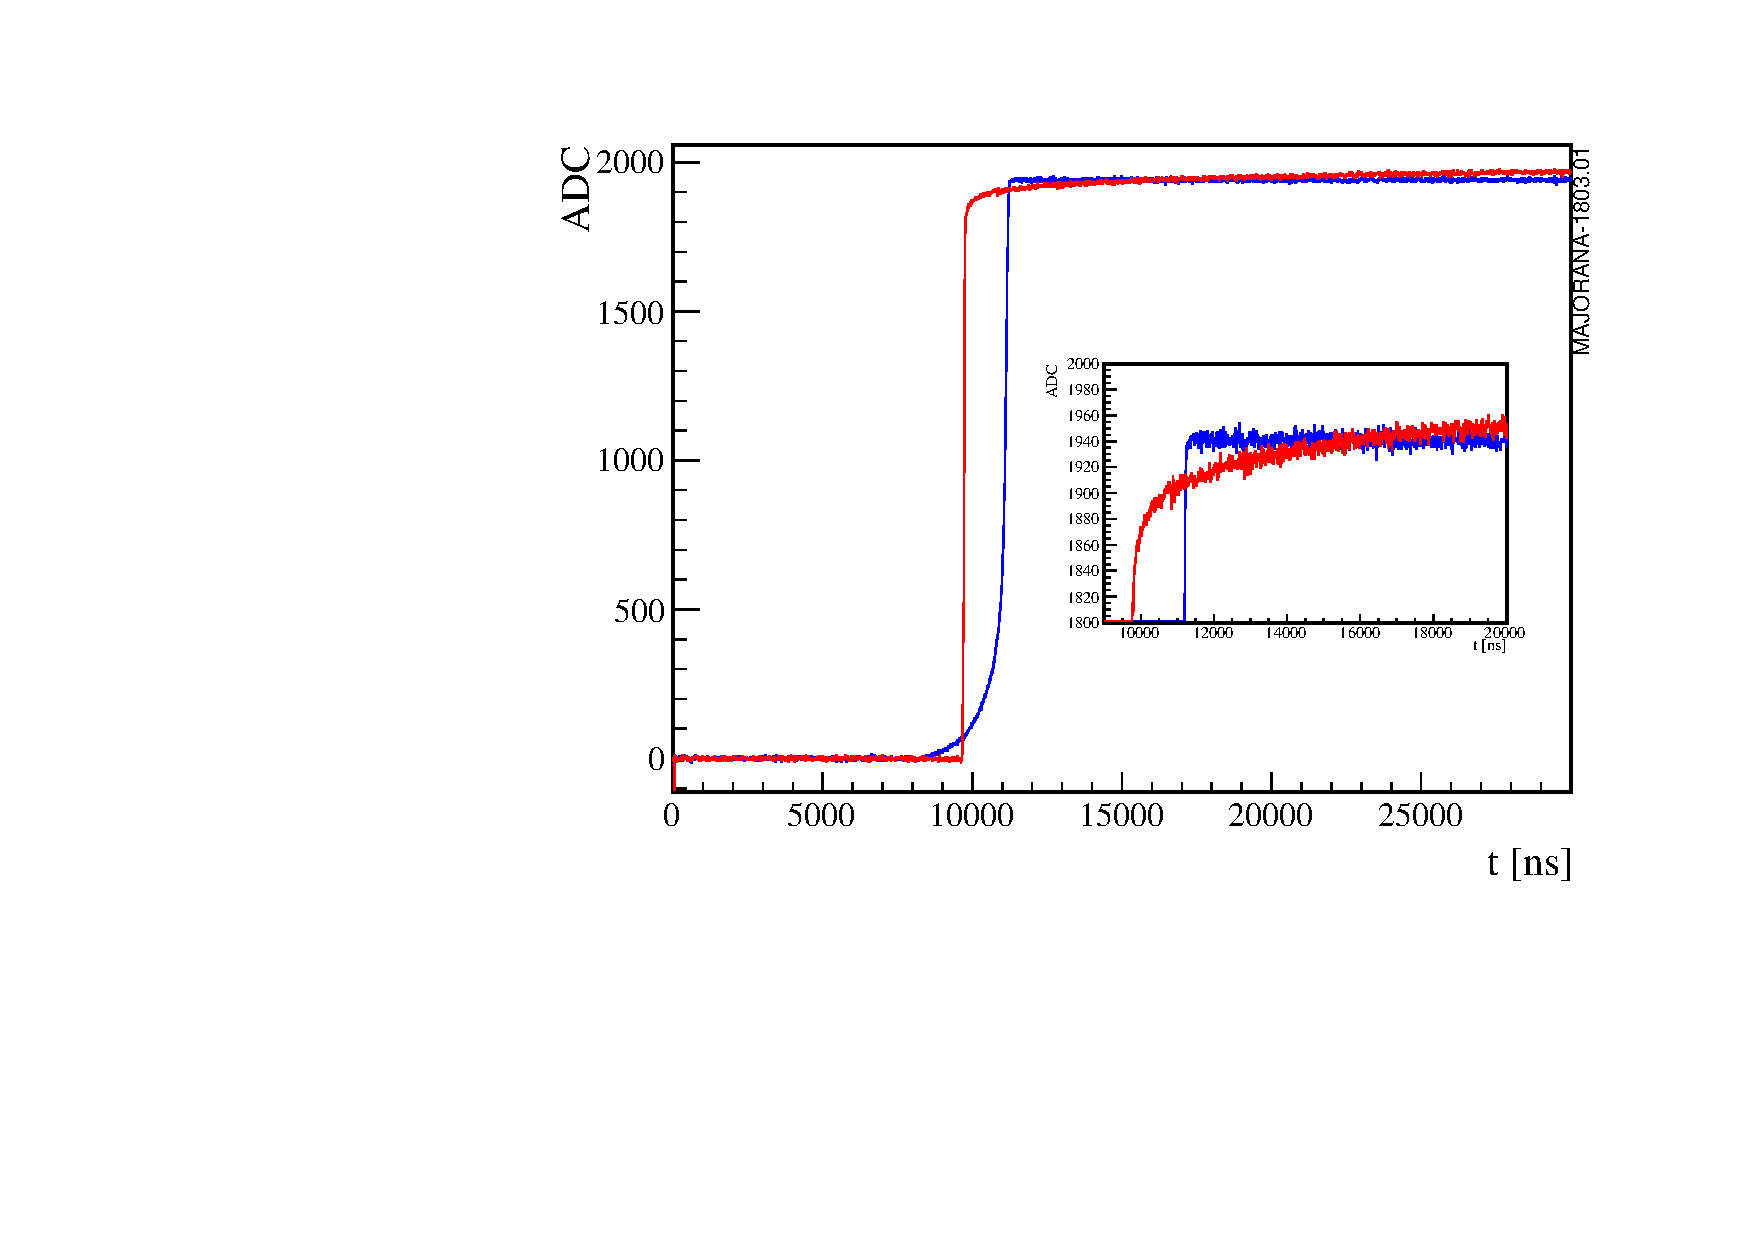
\includegraphics[width=0.8\linewidth]{ch3/figs/dcr_waveform.pdf}
 \caption{An alpha waveform (red) compared to a bulk waveform (blue) in the MJD PPC detector. The DCR effect results in a distinct tail with a smaller slope, as shown by the highlight area in the box.\cite{tube_paper}}
\label{fig:dcr_waveform}
  \end{figure}

The energy of a waveform is measured by applying a filter such as a trap or CUSP filter. This DCR effect means that the filter pickoff will result in energy degradation in the alpha signal. Even though alphas are normally deposited with $5$ MeV energy, the degraded energy could lead alpha events potentially appearing in the ROI. Fig. \ref{ch3_fig_L200_surface_background} shows the {\Ltwo} physics spectrum. Muon and multiplicity cuts remove backgrounds such as muons and gamma rays, and the events left are primarily surface events background in grey. This spread-out spectrum is due to alphas from the DCR effect. As shown in green, Pulse Shape Discrimination (PSD) cuts are highly effective in removing them, but the unknown efficiency of those cuts introduces uncertainty in the background model. 

  \begin{figure}[!htb]
\centering
  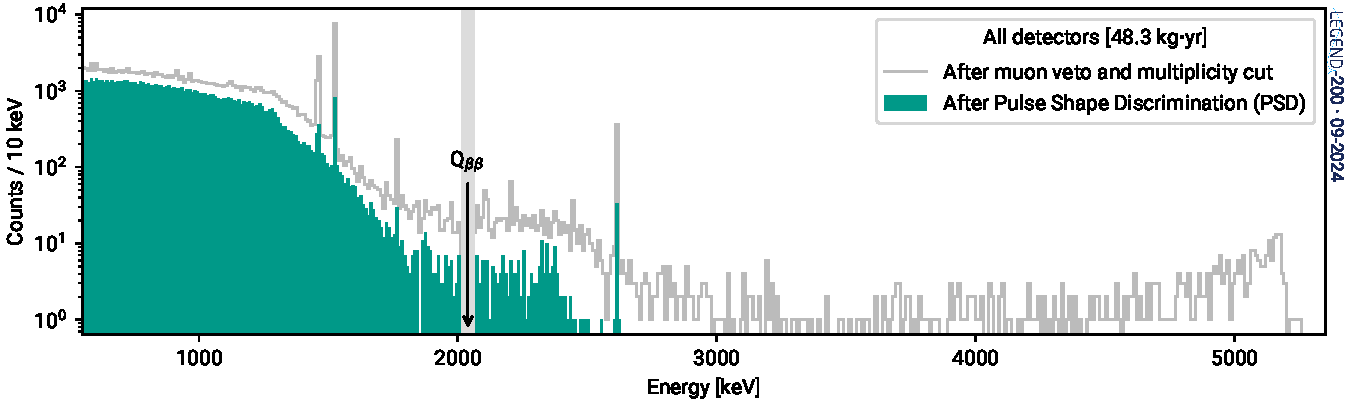
\includegraphics[width=0.99\linewidth]{ch2/figs/l200-phy-spectrum-psd.pdf}
  \caption{{\Ltwo} physics spectrum. The events above 3000 keV after the muon and multiplicity cut are primarily alphas. These events can be effectively remove using PSD cuts as show in green. Credit: Luigi Pertoldi.}
\label{ch3_fig_L200_surface_background}
  \end{figure}

\section{Surface Charge Effect}
Due to various factors such as manufacturing, experimental conditions, and transportation, the HPGe detectors can develop a static charge on the passivated surface which impacts charge collection for surface events. Fig. \ref{ch3_fig_surface_field_sc0} shows how the presence of surface charge alters the electric field close to the passivated surface. When there is no surface charge (top), the field lines are parallel to the surface. The presence of negative surface charge (middle) attracts the field lines towards the surface. Positive surface charge (bottom) repels the field lines from the surface. Negative surface charge can pull the holes to the surface where they can drift slowly. Similarly, positive surface charges can pull the electrons to the surface.

% \clearpage
\begin{figure} %[!htb]
\centering
%[trim={left bottom right top},clip]
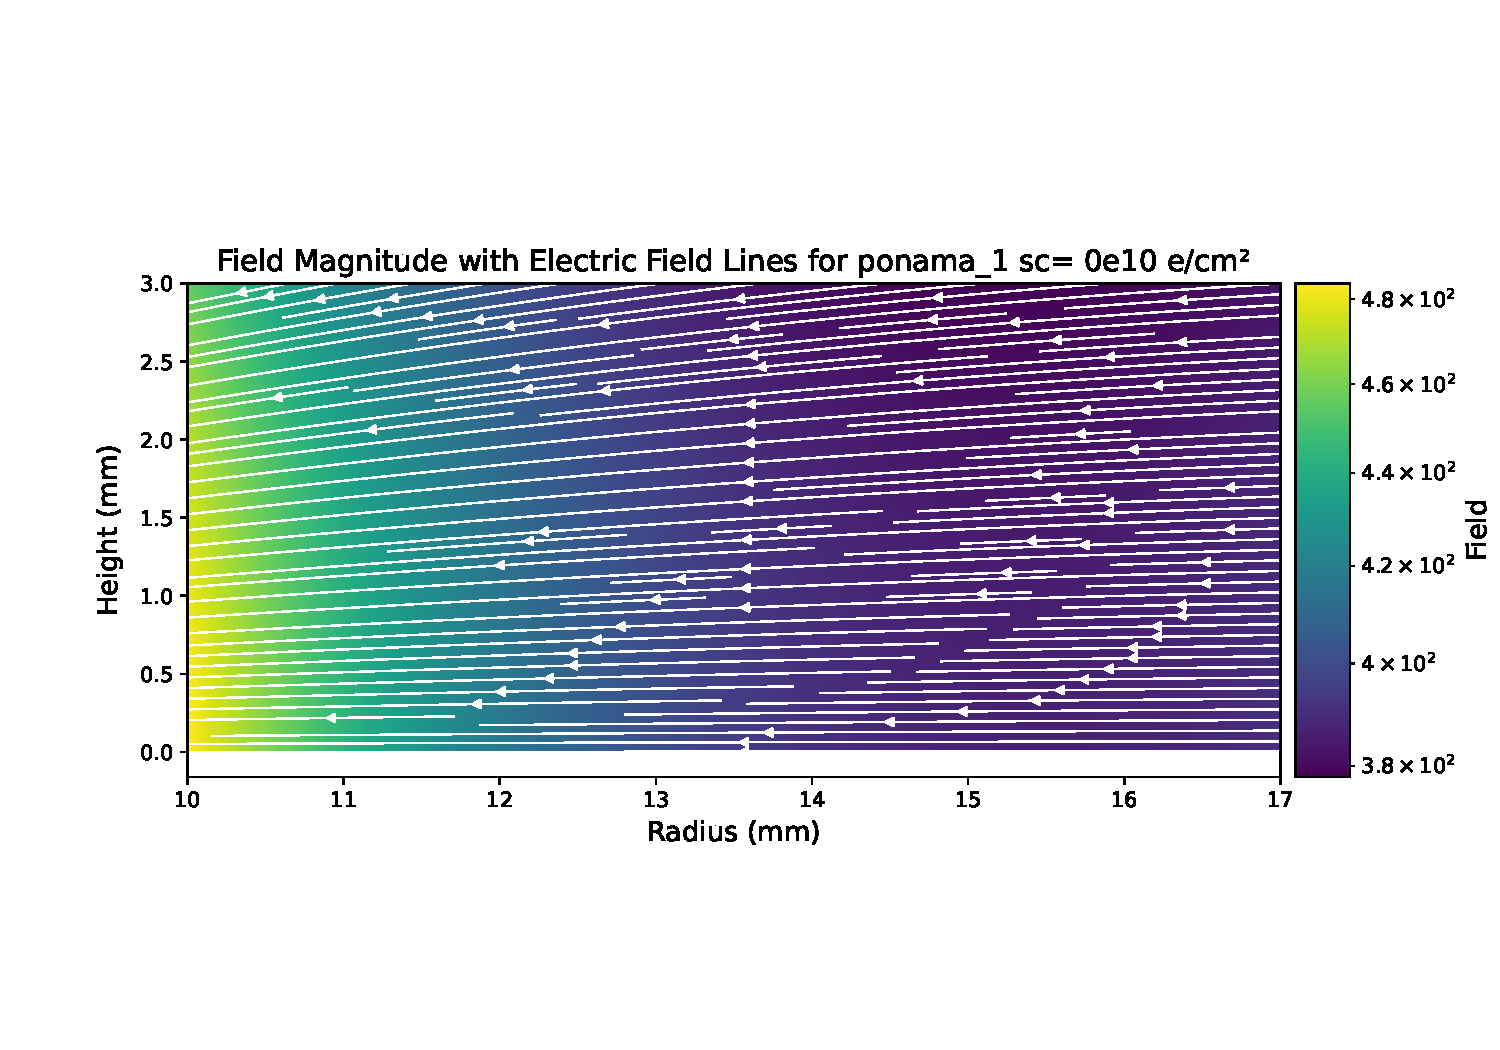
\includegraphics[trim={1cm 3.5cm 0.5cm 4.0cm},clip,width=0.99\linewidth]{ch3/figs/elect_field_lines_surface_ponama_1_sc_0.pdf}
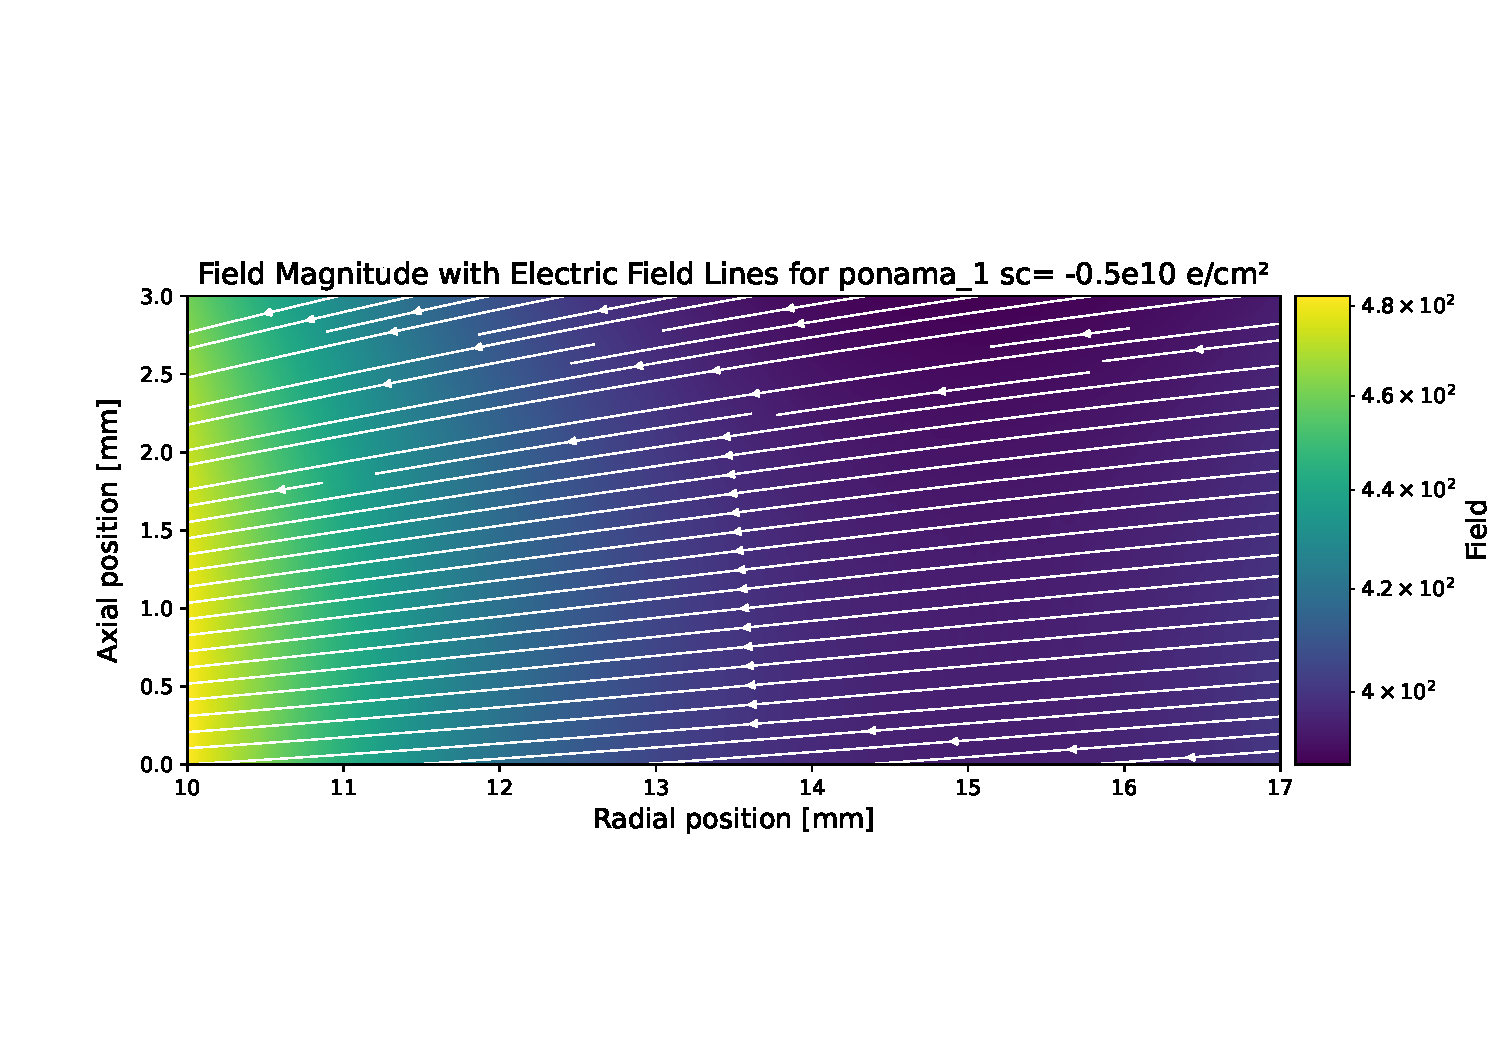
\includegraphics[trim={1cm 3.5cm 0.5cm 4.0cm},clip,width=0.99\linewidth]{ch3/figs/elect_field_lines_surface_ponama_1_sc_-0.5.pdf}
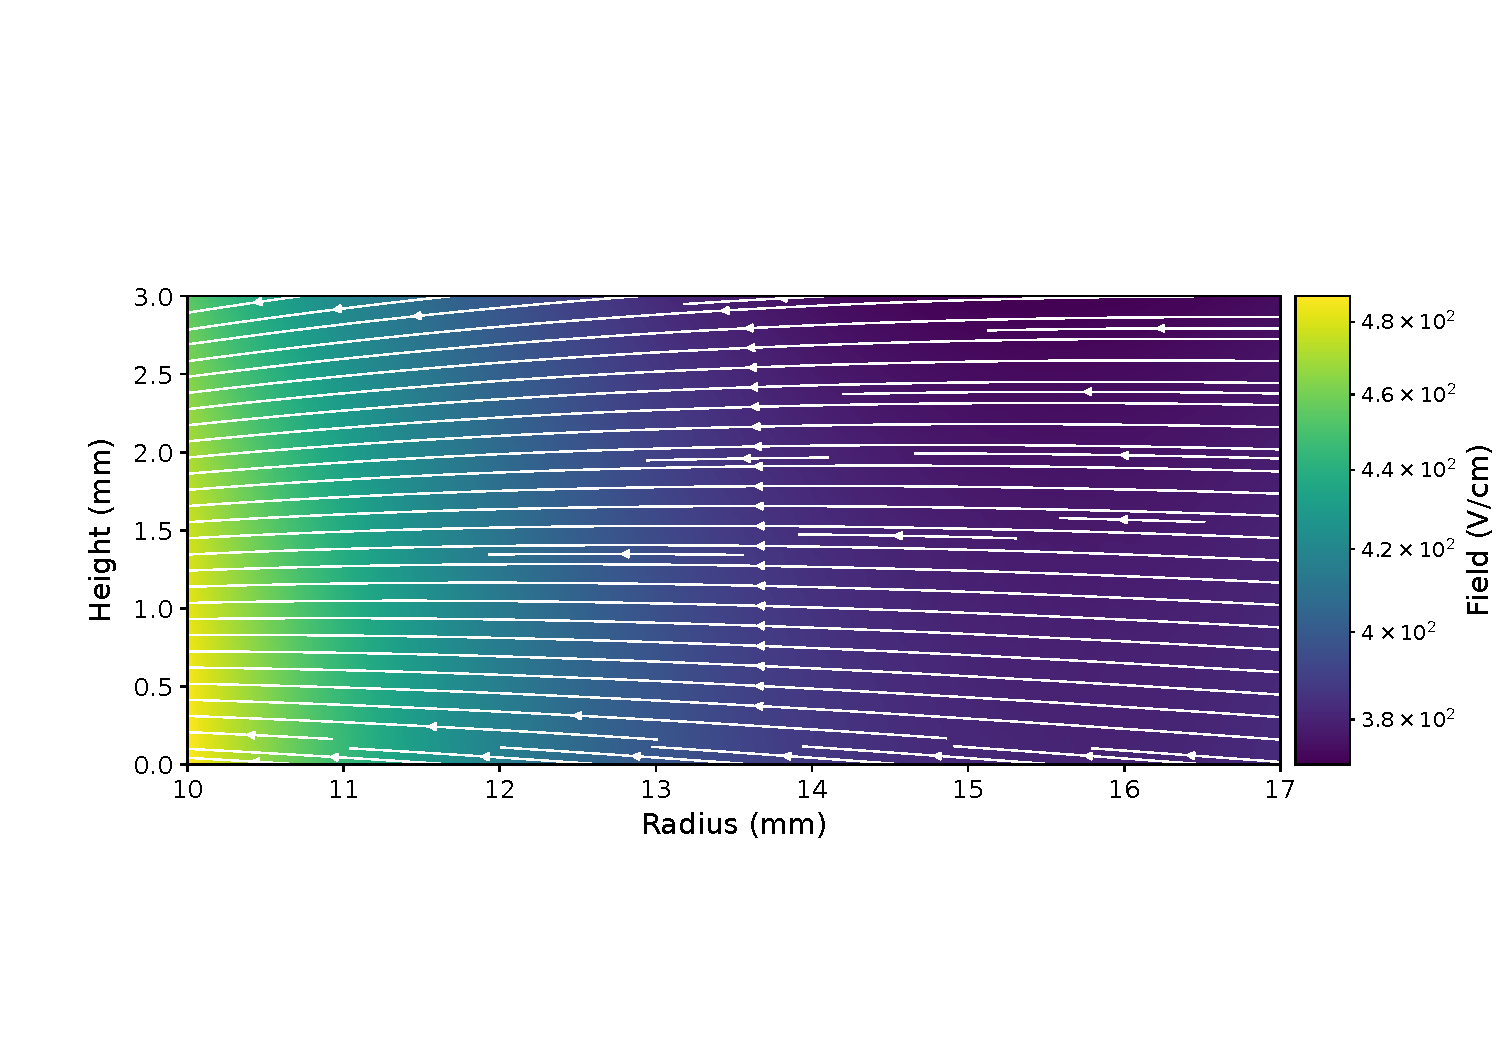
\includegraphics[trim={1cm 3.5cm 0.5cm 4.0cm},clip,width=0.99\linewidth]{ch3/figs/elect_field_lines_surface_ponama_1_sc_0.5.pdf}
\caption{Electric field magnitude and lines for the passivated surface of a PPC detector with different surface charges. Surface charge can pull electrons and holes to the surface and cause additional DCR effects.}
\label{ch3_fig_surface_field_sc0}
\end{figure}


Since surface charge changes the overall electric field of the detector, it could also alter the depletion voltage for the detector. Fig. \ref{ch3_fig_deplection_sc} shows how the depletion voltage for a LEGEND PPC detector changes with surface charge. Typically, the detector's operational voltage is higher than the depletion voltage, but if the surface charges are not properly accounted for, a detector could become depleted after being deployed in the experiment.

\begin{figure}[!htb]
\centering
  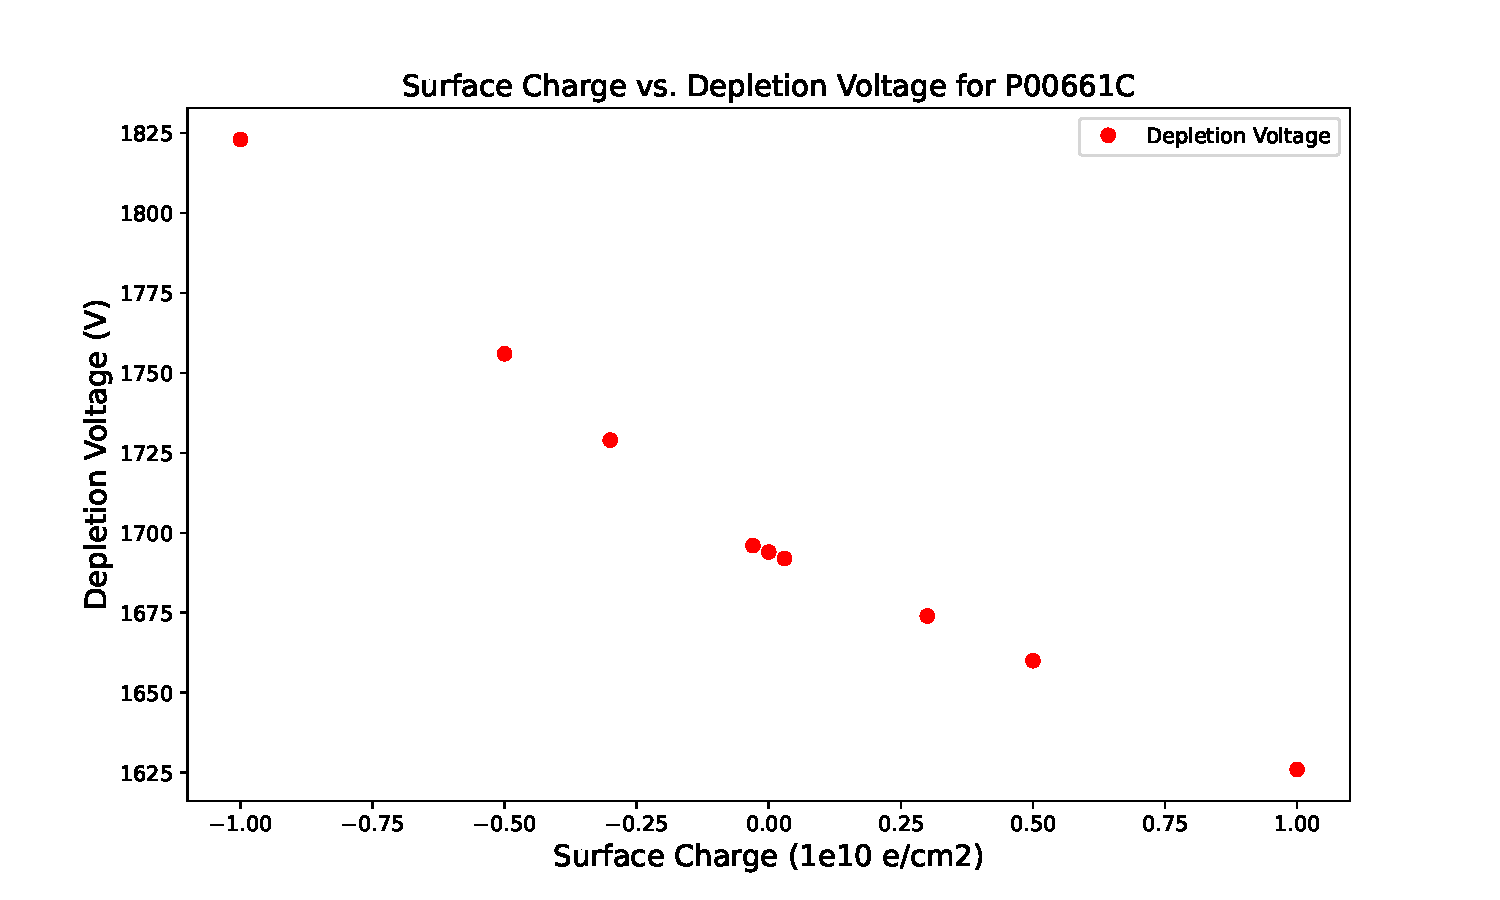
\includegraphics[width=0.99\linewidth]{ch3/figs/deplep_sc.pdf}
 \caption{Effect of surface charge on depletion voltage for LEGEND PPC detector. Depletion voltages calculated using {\siggen} software.}
\label{ch3_fig_deplection_sc}
  \end{figure}

Pulse-shaped simulations can help accurately model these effects and build a background model for surface events. A simulation to model surface events should allow for a nonspherical charge cloud while incorporating surface drift, diffusion, and self-repulsion. They should also properly account for surface charge effects. Next, we look at the current pulse shape simulation frameworks being used by LEGEND.

\section{Pulse shape simulations till now}

Signal formation in Germanium is well understood via the Shockley-Ramo theorem. This enables building accurate simulations that can model the waveforms. Simulations within the LEGEND collaboration include {\siggen} and \texttt{SSD} simulations. 

{\siggen} is a C-based program initially developed by David Radford at Oak Ridge National Lab for MJD pulse shape simulations \cite{siggen_paper}. It consists of two components: \texttt{fieldgen} and {\siggen}. \texttt{fieldgen} is used to calculate the electric potential and weighting potential of point-contact detectors in two-dimensional cylindrical coordinates. The {\siggen} part uses the weighting potential calculated from \texttt{fieldgen} to generate a signal using the Shockley–Ramo theorem. The simulations can also calculate the depletion voltage, the volume of the depletion region, and the capacitance of the detector. Diffusion in {\siggen} is approximated using a Gaussian convolution, and there is no mechanism to account for the self-repulsion of charges as {\siggen} uses point charges to represent the entire charge cloud. {\siggen} has been crucial in LEGEND detector design and manufacturing as it allows precise modeling of electric fields and PSD performance.

% A simulated event in {\siggen} is shown in Fig. \ref{fig:{\siggen}_1d}.

% \begin{figure}
% \centering
% 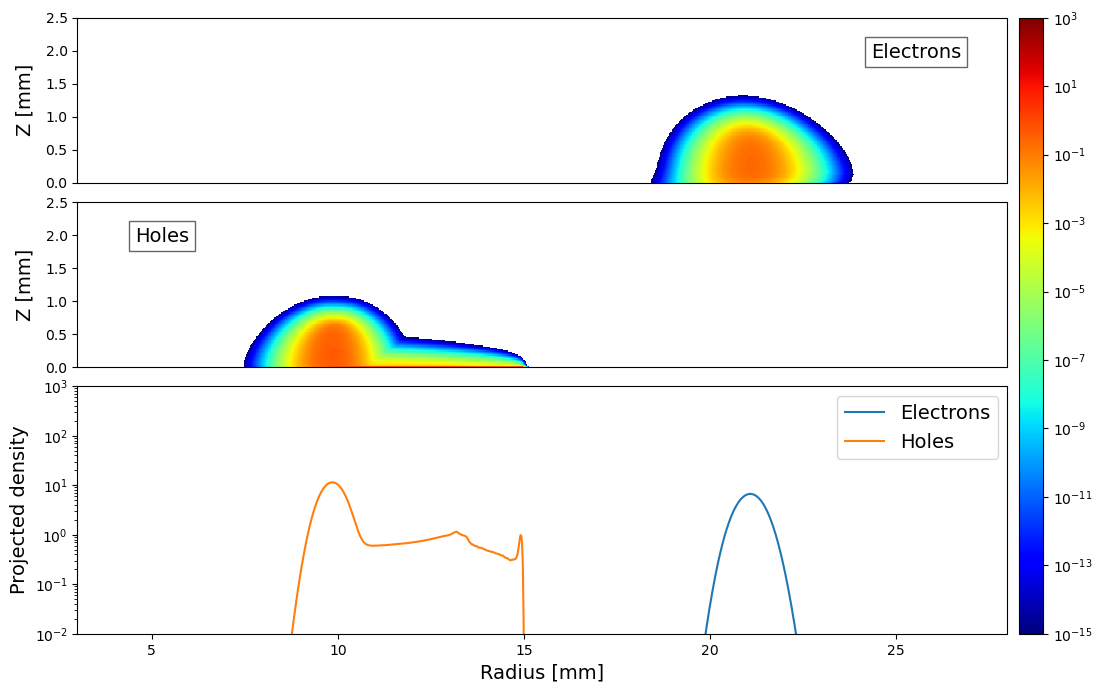
\includegraphics[width=0.49\linewidth]{ch3/figs/drift_path.png}
% 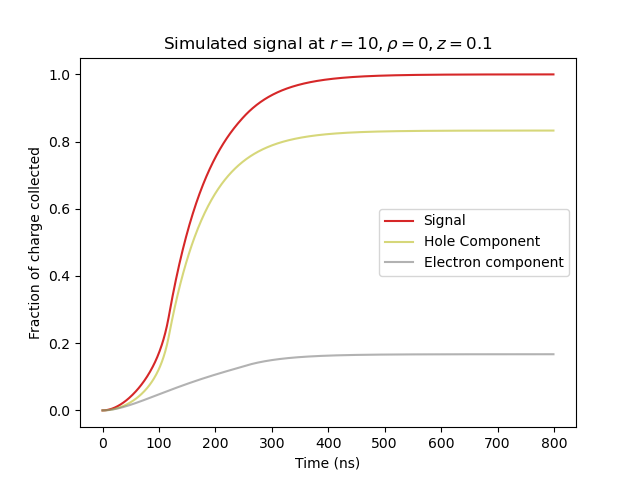
\includegraphics[width=0.49\linewidth]{ch3/figs/samp_wav_comp.png}
% \caption{A simulated event showing the path of holes and electrons and the corresponding waveform}.
% \label{fig:{\siggen}_1d}
% \end{figure}

SolidStateDetectors.jl (\texttt{SSD}) is a software package developed by the group of Iris Abt at the Max Planck Institute Munich for the LEGEND experiment \cite{Abt:2021SSD}. It is written in Julia and can perform calculations in all 3 dimensions. \texttt{SSD} can calculate electric fields and potentials outside the detectors and also has the ability for parallelization. The \texttt{SSD} enables full 3-D diffusion and models self-repulsion in the signal. The charges are tracked individually using their position and velocity. The electric field calculation is done on GPUs. SSD provides a complete 3-D simulation of the charges in Germanium along with surface drift, but the computational run time quickly scales with the number of particles used. Alpha particles typically create a large charge cloud with a number of particles that would be difficult to model with the \texttt{SSD}.

% In bulk, spherical charge cloud model works very well, but the charge cloud produced by alpha is not necessarily spherical due to the charge trapping and re-release effect on the passivated surface. A simulation to model alpha should allow for a nonspherical charge cloud while incorporating surface drift, diffusion, and self-repulsion.

% \begin{figure}
% \centering
% \includegraphics[width=0.49\linewidth]{ch3/figs/\texttt{SSD}_e.png}
% \includegraphics[width=0.49\linewidth]{ch3/figs/\texttt{SSD}_path.png}
% \caption{Simulated Electric field and charge paths in \texttt{SSD} simulations. It allows for calculations outside the detectors and in full 3 dimensions. \cite{\texttt{SSD}_web}.}
% \label{fig:\texttt{SSD}_plots}
% \end{figure}


\section{{\ehd}}
{\ehd} is a method to simulate surface events while directly simulating diffusion and self-repulsion effects. They are a specialized model for surface interactions. The model uses 2-D approximations to optimize run time while adjusting for 3-D effects. They were developed in C by David Radford and built upon {\siggen}. As charges drift through the detectors, they keep track of charge densities at a pixel-by-pixel level, which allows for nonspherical charge clouds. The charges that end up on the surface have their velocities reduced by a predetermined factor. {\ehd} also enables the simulation of the effects of surface charges. The simulation is performed in the r and z-directions while assuming $\phi$ symmetry—thus the charge cloud is simulated by a ring and accounted for the 3-D effects using approximations. The charges that end up on the surface have their velocities reduced by a predetermined factor.

Inspired by Fluid mechanics, {\ehd} take the Lagrangian Splitting approach. This means that each step, such as diffusion, charge drift, etc., is solved independently, and then the net effect is calculated by combining them. Fig. \ref{fig:ehd_flowchart} shows how the {\ehd} program works. The detector is divided into a grid, and charge densities are distributed at a given location based on the impact energy, usually over two adjacent grid points. The initial densities are determined using:

\begin{equation}
    \rho_H = \rho_E= \frac{\text{ E}\times 10^7 }{1000 \times 0.003 \times \text{grid}^3}
\end{equation}

where $\rho$ represents the charge pair density in units of \(10^{10}/\text{cm}^3\). The deposited energy E is the deposited energy in keV, which is first converted to MeV by dividing by 1000.0. The factor of \(10^7\) is to get the final unit correct. The approximate energy required to generate an electron-hole pair in Germanium is \(0.003\). Finally, dividing by \(\text{grid}^3\) normalizes the number of generated charge pairs to the grid volume. The densities for both holes and electrons are deposited equally in points (z,r) and (z+1,r). The density is then multiplied by a factor to get the self-repulsion effect to match the 3-D model. The factor we found was 20.

The boundary conditions are set according to the detector geometry, impurity concentration, surface charge, and bias voltage. Then electric potential and weighting potential are calculated using an over-relaxation algorithm. The capacitance and depletion are estimated. Undepleted regions of a semiconductor detector have no net space charge and no electric field and are indicated by a local minimum in the electrical potential. The capacitance is calculated by relating two equations for the energy stored in a capacitor.

\begin{equation}\label{capacitance_eq}
C= \frac{\epsilon}{V^2} \int_{}^{} E^2 dA
\end{equation}

\begin{figure}[!htb]
\centering
%[trim={left bottom right top},clip]
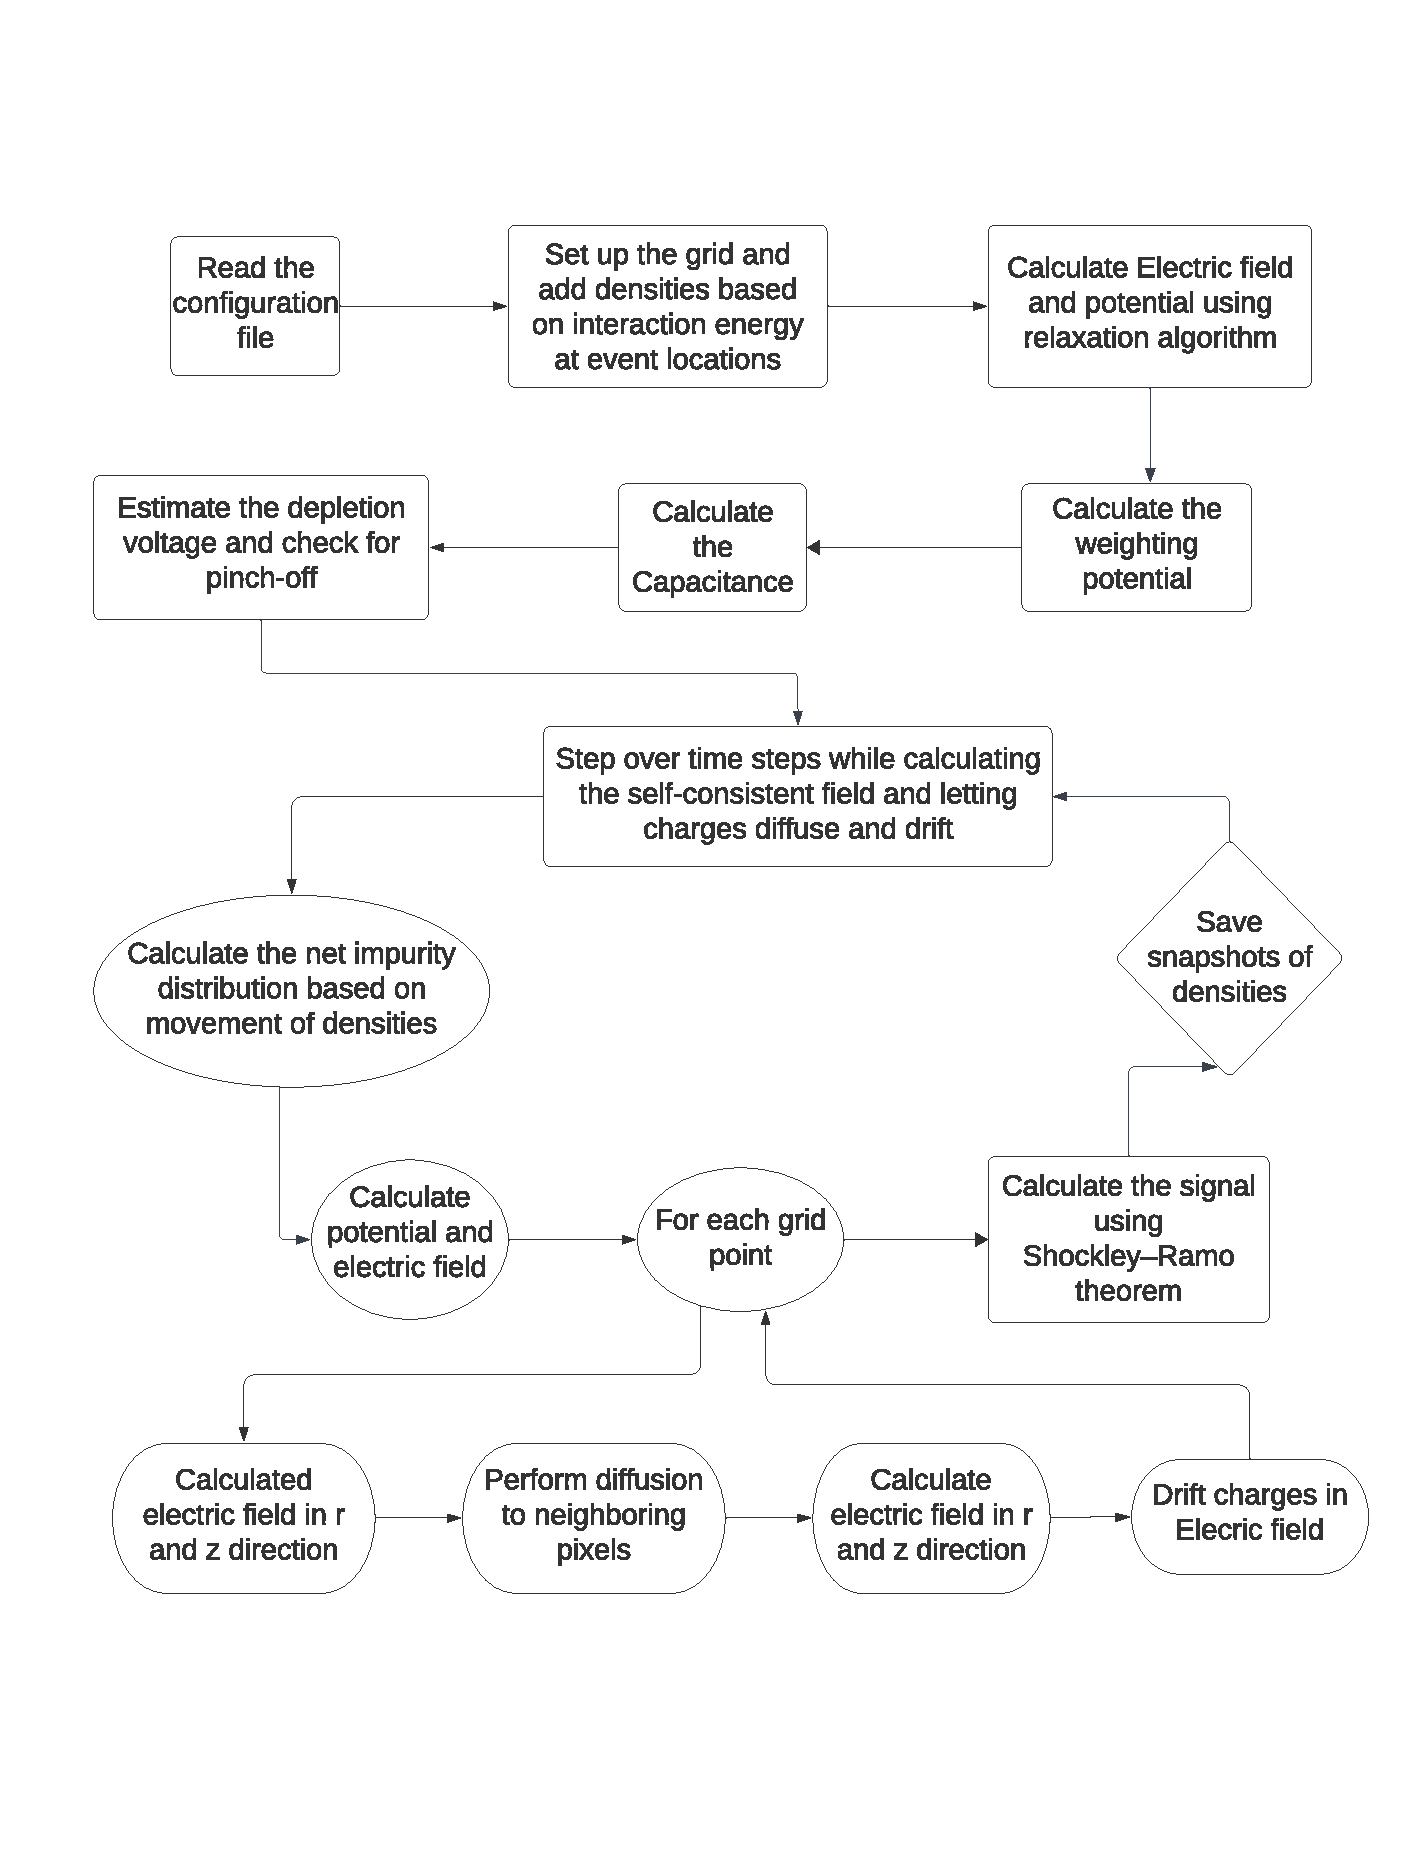
\includegraphics[width=0.99\linewidth,trim={2pc 10pc 1.5pc 9pc},clip]{ch3/figs/ehd_flowchart.pdf}
\caption{A flow chat illustration the pseudo code for {\ehd}.}
\label{fig:ehd_flowchart}
\end{figure}


After the initial setup, the program steps through a small time step. The charges are allowed to diffuse and then drift in the electric field. The calculation of the electric field is discussed in the next chapter. Below we go over some critical components of the {\ehd}.


\section{Diffusion}
Diffusion arises from random thermal motion of electrons and holes, causing them to spread out from regions of high concentration into regions of lower concentration. In thermal equilibrium, the diffusion coefficient $D$ and the mobility $\mu$
are related by the Einstein relation:
\begin{equation}
D = \mu \frac{k_B T}{q},
\end{equation}
where $k_B$ is Boltzmann's constant, $T$ is the absolute temperature, and $q$ is the elementary charge. Thus, if the mobility $\mu$ is known or has been fit to experimental data, $D$ may be determined for a specified temperature. In germanium at cryogenic temperatures (e.g., $\sim 77$\,K), the mobilities are
sufficiently large that diffusion can still have a noticeable effect on the final spread of a charge cloud, although it is smaller compared to room temperature conditions.


In {\ehd} the diffusion is simulated by redistributing charge among neighboring grid cells in $(r)$ and $(z)$ directions using the diffusion coefficients. During each time step $\Delta t$, a fraction of the carriers in cell $(z,r)$ diffuse to the adjacent cells $(z\pm1,\,r\pm1)$ according to two quantities: $\delta_z$ and $\delta_r$. These fractions are computed from an approximate diffusion parameter $f$ and the local drift velocity magnitudes $\lvert \mathbf{v_z} \rvert$, $\lvert \mathbf{v_r} \rvert$ as follows:
\begin{align}
   \delta_z &\;=\; \frac{\Delta x \;\,v_z \;f}{E_z}\label{eq:deltaez}\\
   \delta_r &\;=\; \frac{\Delta x \;\,v_r \;f}{E_r} \label{eq:deltaer}
\end{align}
where $\Delta x$ is the grid size, $v_{z}$ and $v_{r}$ are the drift velocities, $E_{z}$ and $E_{r}$ are the local field components, and $f$ incorporates the diffusion coefficient $D$ and corrections for grid sizes. If $E_z$ or $E_r$ is below $1\,\mathrm{V/cm}$, the program sets $\delta_z = 0$ or $\delta_r=0$ assuming low-field regions produce negligible drift velocity.

\subsection{Volume Correction}

In cylindrical $(r,z)$ coordinates, each radial ring has a different physical area. The simulation tracks these scaling factors with arrays:
\[
\texttt{s1}[r] = 1 + \frac{0.5}{r-1}, 
\qquad
\texttt{s2}[r] = 1 - \frac{0.5}{r-1},
\] 

For r=1 and r=0, the code uses a special fixed weighting factor to handle the geometry. These scalars adjust how much charge diffuses into or out of the neighboring ring. Specifically, if $\delta_r$ is the fraction of carriers leaving cell $(r)$ in 
the $+r$ direction, the actual increment in the neighbor cell 
$(r+1)$ is multiplied by $\texttt{s1}[r]$, while the old cell is 
reduced by the same fraction multiplied by $\texttt{s1}[r]$ to 
balance volume differences. Similarly, diffusion to cell $(r-1)$ 
uses $\texttt{s2}[r]$. The same volume correction is used in field calculation.

\section{Diffusion Density Update}

After computing the diffusion fractions $\delta_z$ and $\delta_r$, the code subtracts those amounts from the point's density and adds them to the four neighbors:
\begin{align}
  \rho^{\mathrm{new}}(z,\,r+1) &\;\mathrel{+}= \;\rho^{\mathrm{old}}(z,\,r)\times\delta_r \times s_1(r) \times \frac{r-1}{r} \label{ch3:eq:diffusion_update_1} \\
  \rho^{\mathrm{new}}(z-1,\,r) &\;\mathrel{+}= \;\rho^{\mathrm{old}}(z,\,r)\times\delta_z \label{ch3:eq:diffusion_update_2} \\
  \rho^{\mathrm{new}}(z+1,\,r) &\;\mathrel{+}= \;\rho^{\mathrm{old}}(z,\,r)\times\delta_z \label{ch3:eq:diffusion_update_3} \\
  \rho^{\mathrm{new}}(z,\,r-1) &\;\mathrel{+}= \;\rho^{\mathrm{old}}(z,\,r) \times \delta_r \times s_2(r) \times\frac{r-1}{r-2} \label{ch3:eq:diffusion_update_4}.
\end{align}
 The offsets $r$ and $r-2$ are due to one-based indexing in the code.
 
\section{Drift in Electric Field}
Germanium has a diamond cubic lattice structure. The crystallographic basis axes are in $<h100>$, $<h110>$, and $<h111>$ directions. Charges in the three basis axes travel at different velocities. Mobility relates the velocity of the charges to the electric field. At low field, the relationship is Ohmic:
\begin{equation}
\vec{v} = \mu_0 \vec{E}
\end{equation}
At higher field, the scattering with the crystal lattice results in a nonlinear relationship. This scattering causes the velocity to saturate at higher values. The relationship at higher field can be modeled using \cite{Caughey_1448053}:

\begin{equation}
v(E) = \frac{\mu_0 E}{(1 + (E/E_0)^\beta)^{1/\beta}}
\end{equation}

In {\ehd}, we calculate the electric field in r and z directions at each grid point. We use values from \cite{OMAR19871351} which gives $v(E)$ from the local electric field $E$. We use a piecewise linear interpolation to find the $v(E)$. To do this, we define an array of electric field points, $\texttt{drift\_E}$, which partitions the field range into intervals. For each interval $[E_i, E_{i+1}]$, we store two quantities: a drift offset, corresponding to the drift velocity at $E = E_i$, and a drift slope, which is the rate of change of drift velocity with respect to the electric field in that interval. The drift velocity is then
computed by:
\[
v(E) \;=\; \text{drift offset}[i]
\;+\; \text{drift slope}[i] \,\bigl( E - E_i \bigr),
\]
with $E_i \le E < E_{i+1}$. The fig. \ref{ch3:fig:dv_vs_e} simulates the relation for the Drift Velocity versus Electric field.  For simplicity, we only use the $<100>$ direction velocities in the current model. The drift velocity is then multiplied by the time step to find where the charges will drift, and then the charges are moved to the new location.

\begin{figure}[!htb]
    %[trim={left bottom right top},clip]
    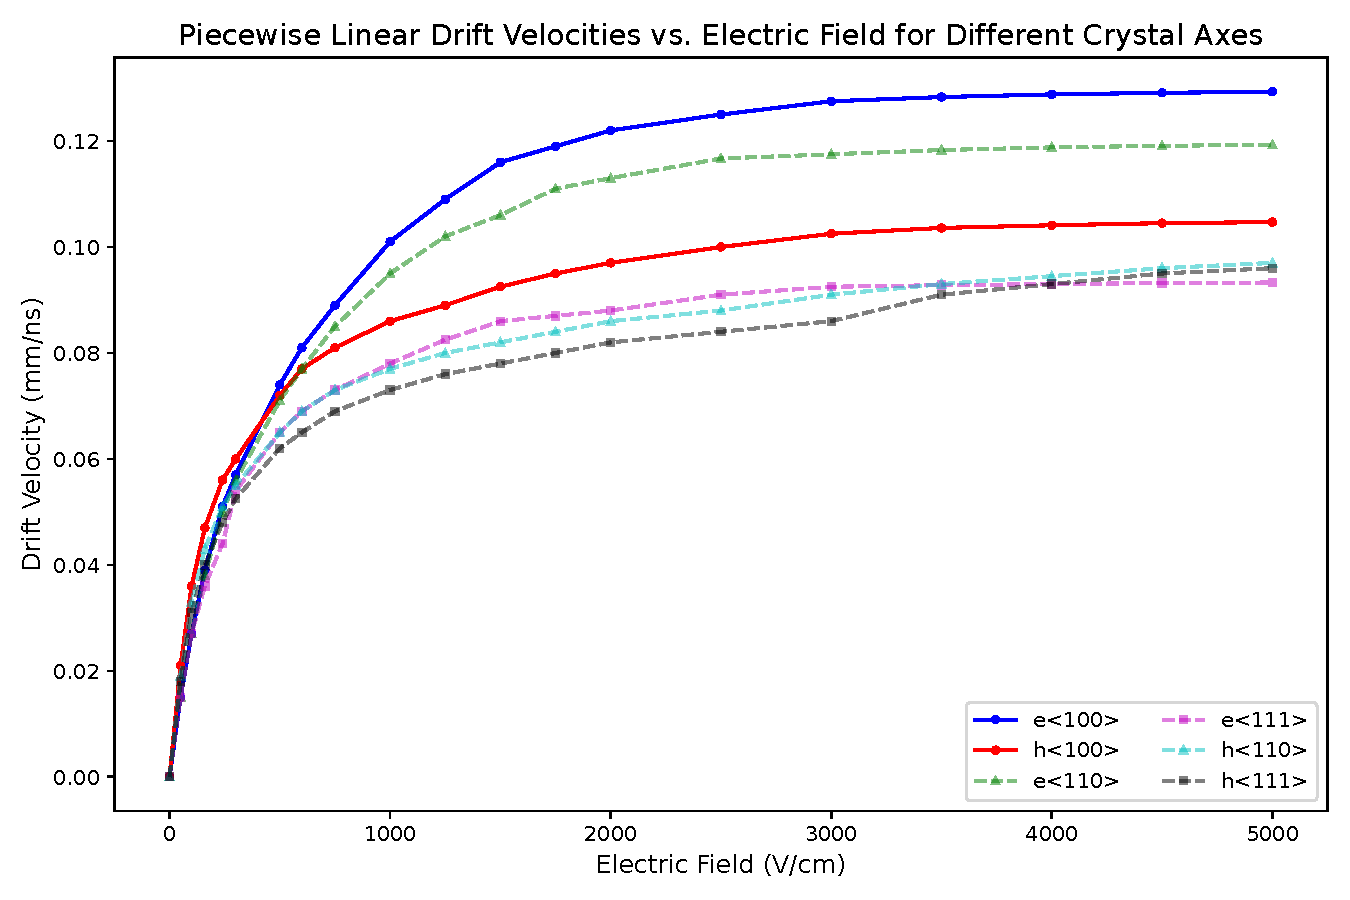
\includegraphics[trim={0cm 0 0cm 0},clip,width=0.99\linewidth]{ch3/figs/ehd_dv_e.pdf}
    \caption{Relation of drift velocity verses electric field in {\ehd}. The points shows the experimental values are adapted from \cite{OMAR19871351}. To show how {\ehd} estimates the values we create 500 samples between 0 and 5000 V/cm and performed the piecewise linear interpolation between the points. Only $<100>$ direction velocities are used in the current model.}
    \label{ch3:fig:dv_vs_e}
\end{figure}

\subsection{Fraction Splitting}\label{ch3:sec:frac_split}
We use a splitting approach to move the charges to the new cell. Since we are using a grid, we want to account for the discretization by splitting the charges between two grid points. Suppose that after a time step $\Delta t$, the density in grid cell $(z,r)$ moves to a new position with integer indices $(k,i)$. We define fractional parts $f_z$ and $f_r$ as:
%
\begin{align}
k \;=\; z + \lfloor \Delta z \rfloor,\quad
f_z \;=\; \Delta z - \lfloor \Delta z \rfloor,\\
i \;=\; r + \lfloor \Delta r \rfloor,\quad
f_r \;=\; \Delta r - \lfloor \Delta r \rfloor,
\end{align}


The charges are split using these fractions:
\begin{align}
&\text{fraction in }(k, i)   \;=\; f_{r} \times f_{z} \\
&\text{fraction in }(k, i+1) \;=\; (1 - f_{r}) \times f_{z}\\
&\text{fraction in }(k+1, i) \;=\; f_{r} \times (1 - f_{z})\\
&\text{fraction in }(k+1, i+1)\;=\; (1 - f_{r}) \times (1 - f_{z}).
\label{eq:bilinear-fractions}
\end{align}

Finally, the densities are updated using:
\begin{align}
\rho^{\mathrm{new}}(k,i)   &\,\mathrel{+}=\, \rho^{\mathrm{old}}(z,r)\times \bigl[f_{r}\times f_{z}\bigr] \times \text{G}_{r,z} \label{ch3:eq:den_update_1} \\
\rho^{\mathrm{new}}(k,i+1) &\,\mathrel{+}=\, \rho^{\mathrm{old}}(z,r)\times \bigl[(1 - f_{r})\,f_{z}\bigr] \times \text{H}_{r,z} \label{ch3:eq:den_update_2} \\
\rho^{\mathrm{new}}(k+1,i) &\,\mathrel{+}=\, \rho^{\mathrm{old}}(z,r)\times \bigl[f_{r}\,(1 - f_{z})\bigr] \times \text{G}_{r,z} \label{ch3:eq:den_update_3} \\
\rho^{\mathrm{new}}(k+1,i+1)&\,\mathrel{+}=\, \rho^{\mathrm{old}}(z,r)\times \bigl[(1 - f_{r})\,(1 - f_{z})\bigr] \times \text{H}_{r,z}. \label{ch3:eq:den_update_4}
\end{align}
\subsection{Geometric Factors}
\label{sec:geom-factor}

In cylindrical coordinates, each cell at index $r$ corresponds to an annular region of approximate circumference $2\pi (r \,\Delta r)$ and thickness $\Delta z$. When charge moves from cell $(z,r)$ to cell $(k,i)$, we apply the factors:
\[
\text{G}_{r,z} \;\equiv\; \frac{(r-1)}{(i-1)}
\qquad
\text{H}_{r,z} \;\equiv\; \frac{(r-1)}{(i)}
\] 

reflecting the difference in volumes at radii $r$ and $i$.
The offsets $(r-1)$ and $(i-1)$ are for one-based indexing in the code. For the points near $r=0$ or $i=0$, the code uses a modified factor that preserves volume scaling. 

% The factors \verb|8*r - 8| or \verb|8*i - 8| are specialized scalings to approximate the annular volume near the central axis or near $i=0$. They ensure that even when $r$ or $i$ equals 0 or 1, the total charge remains consistent with the expected geometry. For example, at the very center ($r=0$), a full ring circumference does not exist, so a smaller effective volume must be used. Although such \verb|8*-8| scalings can appear ad~hoc, they are designed to smoothly transition from the central axis to the first few radial rings, thereby avoiding division by zero while preserving charge.

\section{Surface Drift}

When charge carriers drift within the detector, they may encounter the passivated surface, which is handled separately. To model the surface, the lowest grid point is split into two lengths: the length of the surface and grid minus the length of the surface. We store the charges on the surface in a special row. 

If the height to which the charges drift is less than zero, they are fully added to the surface row. If the charge enters the passivated layer, we split it up using the fraction splitting described in \ref{ch3:sec:frac_split}. While performing the diffusion on the last grid point in Eq. \ref{ch3:eq:diffusion_update_2}, the bottom z point is considered to be the passivated surface. 


We employ the same methods described above for drifting and diffusing the charges present on the surface, but the drift and diffusion are suppressed by the surface drift velocity factor. This factor, typically about 0.001, is the ratio of the speed on the surface to the bulk. The charges from the surface can drift to the bulk or to other points on the surface. Points on the surface can diffuse up or to other points on the surface.

\section{Courant Number and Adaptive Time Step}

The Courant–Friedrichs–Lewy (CFL) condition is a required condition for numerical solutions of partial differential equations which involve moving particles \cite{cfl_condition}. It is commonly used in fluid dynamics to ensure that particles only travel to the immediate grid points. We introduce the CFL condition in the {\ehd} to ensure that the time step is small enough such that the distance charges drift is not too big during a step. This helps maintain consistency for different input grid sizes. During each time step of simulations, we calculate the local Courant number at every grid point using:

\begin{equation}
C(z,r) = \max \left( \frac{v_r \Delta t}{\Delta x}, \frac{v_z \Delta t}{\Delta x} \right),
\end{equation}

where \( v_r \) and \( v_z \) are the drift velocities in r and z directions, respectively, and  \( \Delta x \) is the grid spacing. The time step is updated using the largest Courant number on the grid :

\begin{equation}
\Delta t = \frac{1}{\max (C(z,r))}.
\end{equation}



\section{Impurity Correction}
Surface events create a large amount of charge carriers that could impact local impurity and must be corrected to accurately calculate the electric potential. At a given time, impurity correction is given by:

\begin{equation}
  {\text{I}_{t}}(z, r) = \text{I}_{0}(z, r) +
  \bigl( \rho_h(z, r) - \rho_e(z, r) \bigr) \times \frac{e}{\epsilon} \times \frac{(\Delta x)^2}{2}.
\end{equation}
The $\text{I}_{0}$ is the impurity of the crystal from production. $\rho_h(z,r)$ and $\rho_e(z,r)$ are the hole and electron densities, respectively. $\frac{e}{\epsilon}$ is the conversion factor that relates charge density to the resulting electric field, derived from Gauss’s law in Germanium with $\epsilon = 16\epsilon_0$. $\frac{e}{\epsilon} = 11.310$ in 
charge units $10^{10}\frac{e}{cm^3}$. $(\Delta x)^2$ is the area of the grid which converts density into charge, and then the conversion factor converts it into $10^{10}\frac{e}{cm^3}$ units to match the units of impurity used.

\section{Signal Calculation}
In cylindrical coordinates, each grid cell at radius $r$ and height $z$ has an approximate area proportional to $(r - 1)$. Once we read the electron 
density $\rho_e(r,z)$ and hole density $\rho_h(r,z)$ at time $t$, the weighted sums are defined as:
\begin{align}
S_e(t) \;=\; \sum_{z=1}^{L-1} \sum_{r=1}^{R-1}
   \rho_e(r,z)\,\bigl(r-1\bigr)\,\text{wpot}[r-1][z-1],\\
S_h(t) \;=\; \sum_{z=1}^{L-1} \sum_{r=1}^{R-1}
   \rho_h(r,z)\,\bigl(r-1\bigr)\,\text{wpot}[r-1][z-1],
\end{align}
where \(\texttt{wpot}[\,r-1\,][\,z-1\,]\) is the weighting potential at that grid 
point. These $S_e(t)$ and $S_h(t)$ represent the induced signal contributions 
from electrons and holes, respectively, via Shockley-Ramo’s theorem.

The initial unweighted sums are defined as:
\begin{align}
R_{e}(0) \;=\; \sum_{z=1}^{L-1} \sum_{r=1}^{R-1}
   \rho_e(r,z)\,\bigl(r-1\bigr), \quad \\
R_{h}(0) \;=\; \sum_{z=1}^{L-1} \sum_{r=1}^{R-1}
   \rho_h(r,z)\,\bigl(r-1\bigr), \quad
\end{align}
% They keep track of how many electrons or holes remain in the crystal at time $t$ 
% (as opposed to how much they contribute to the signal).  For instance, if 
% $R_{h}(t)$ drops below $R_{h}(0)$, that implies some fraction of holes 
% has reached the collecting electrode or left the active region.

Combining these quantities, the induced signal at time t is computed using:
\begin{equation}
\text{Signal}[\,t\,] 
\;=\;
  \frac{\,S_h(t)\;-\;S_h(0)\,}{\,R_{h}(0)\,}
  \;-\;
  \frac{\,S_e(t)\;-\;S_e(0)\,}{\,R_{e}(0)\,}
\label{eq:net-signal}
\end{equation}
Since the electrons’ contribution would be negative, we subtract it from holes to get the net induced signal. Normalizing by $R_{e}(0)$ and $R_{h}(0)$ ensures that the signal is expressed as a fraction of the original total electron/hole count, so it starts near zero at $t=0$ and approaches 1 as all charges arrive at the contacts.

\section{Density Snapshots}

The ability to store snapshots of density at each time step provides detailed information about how the charges drift in the detector. Fig. \ref{ch3_fig_ehd_path_pd_sc_0} shows a snapshot at time=$80$ns in the {\ehd} for a 5 MeV energy deposition close to the surface with no charge. The event started at r=15 mm, and the electron and hole clouds drift towards the respective electrodes.  A 5 MeV energy can create a charge cloud 1.5 mm tall. Charges in such a large charge cloud could drift and diffuse to the surface. The projected density shows the distribution of the charge in the cloud on the x-axis. The head of each signal is the peak, which is where charges would have normally traveled in bulk. The tail of the projected density has a peak that is due to the charges that were initially pushed to the surface. The points in between the two peaks are charges that drifted or diffused to the surface in intermediate steps. The drift on the surface, in this case, is set to be $1000$ slower than drift in bulk. 

\begin{figure}%[!htb]
    %[trim={left bottom right top},clip]
    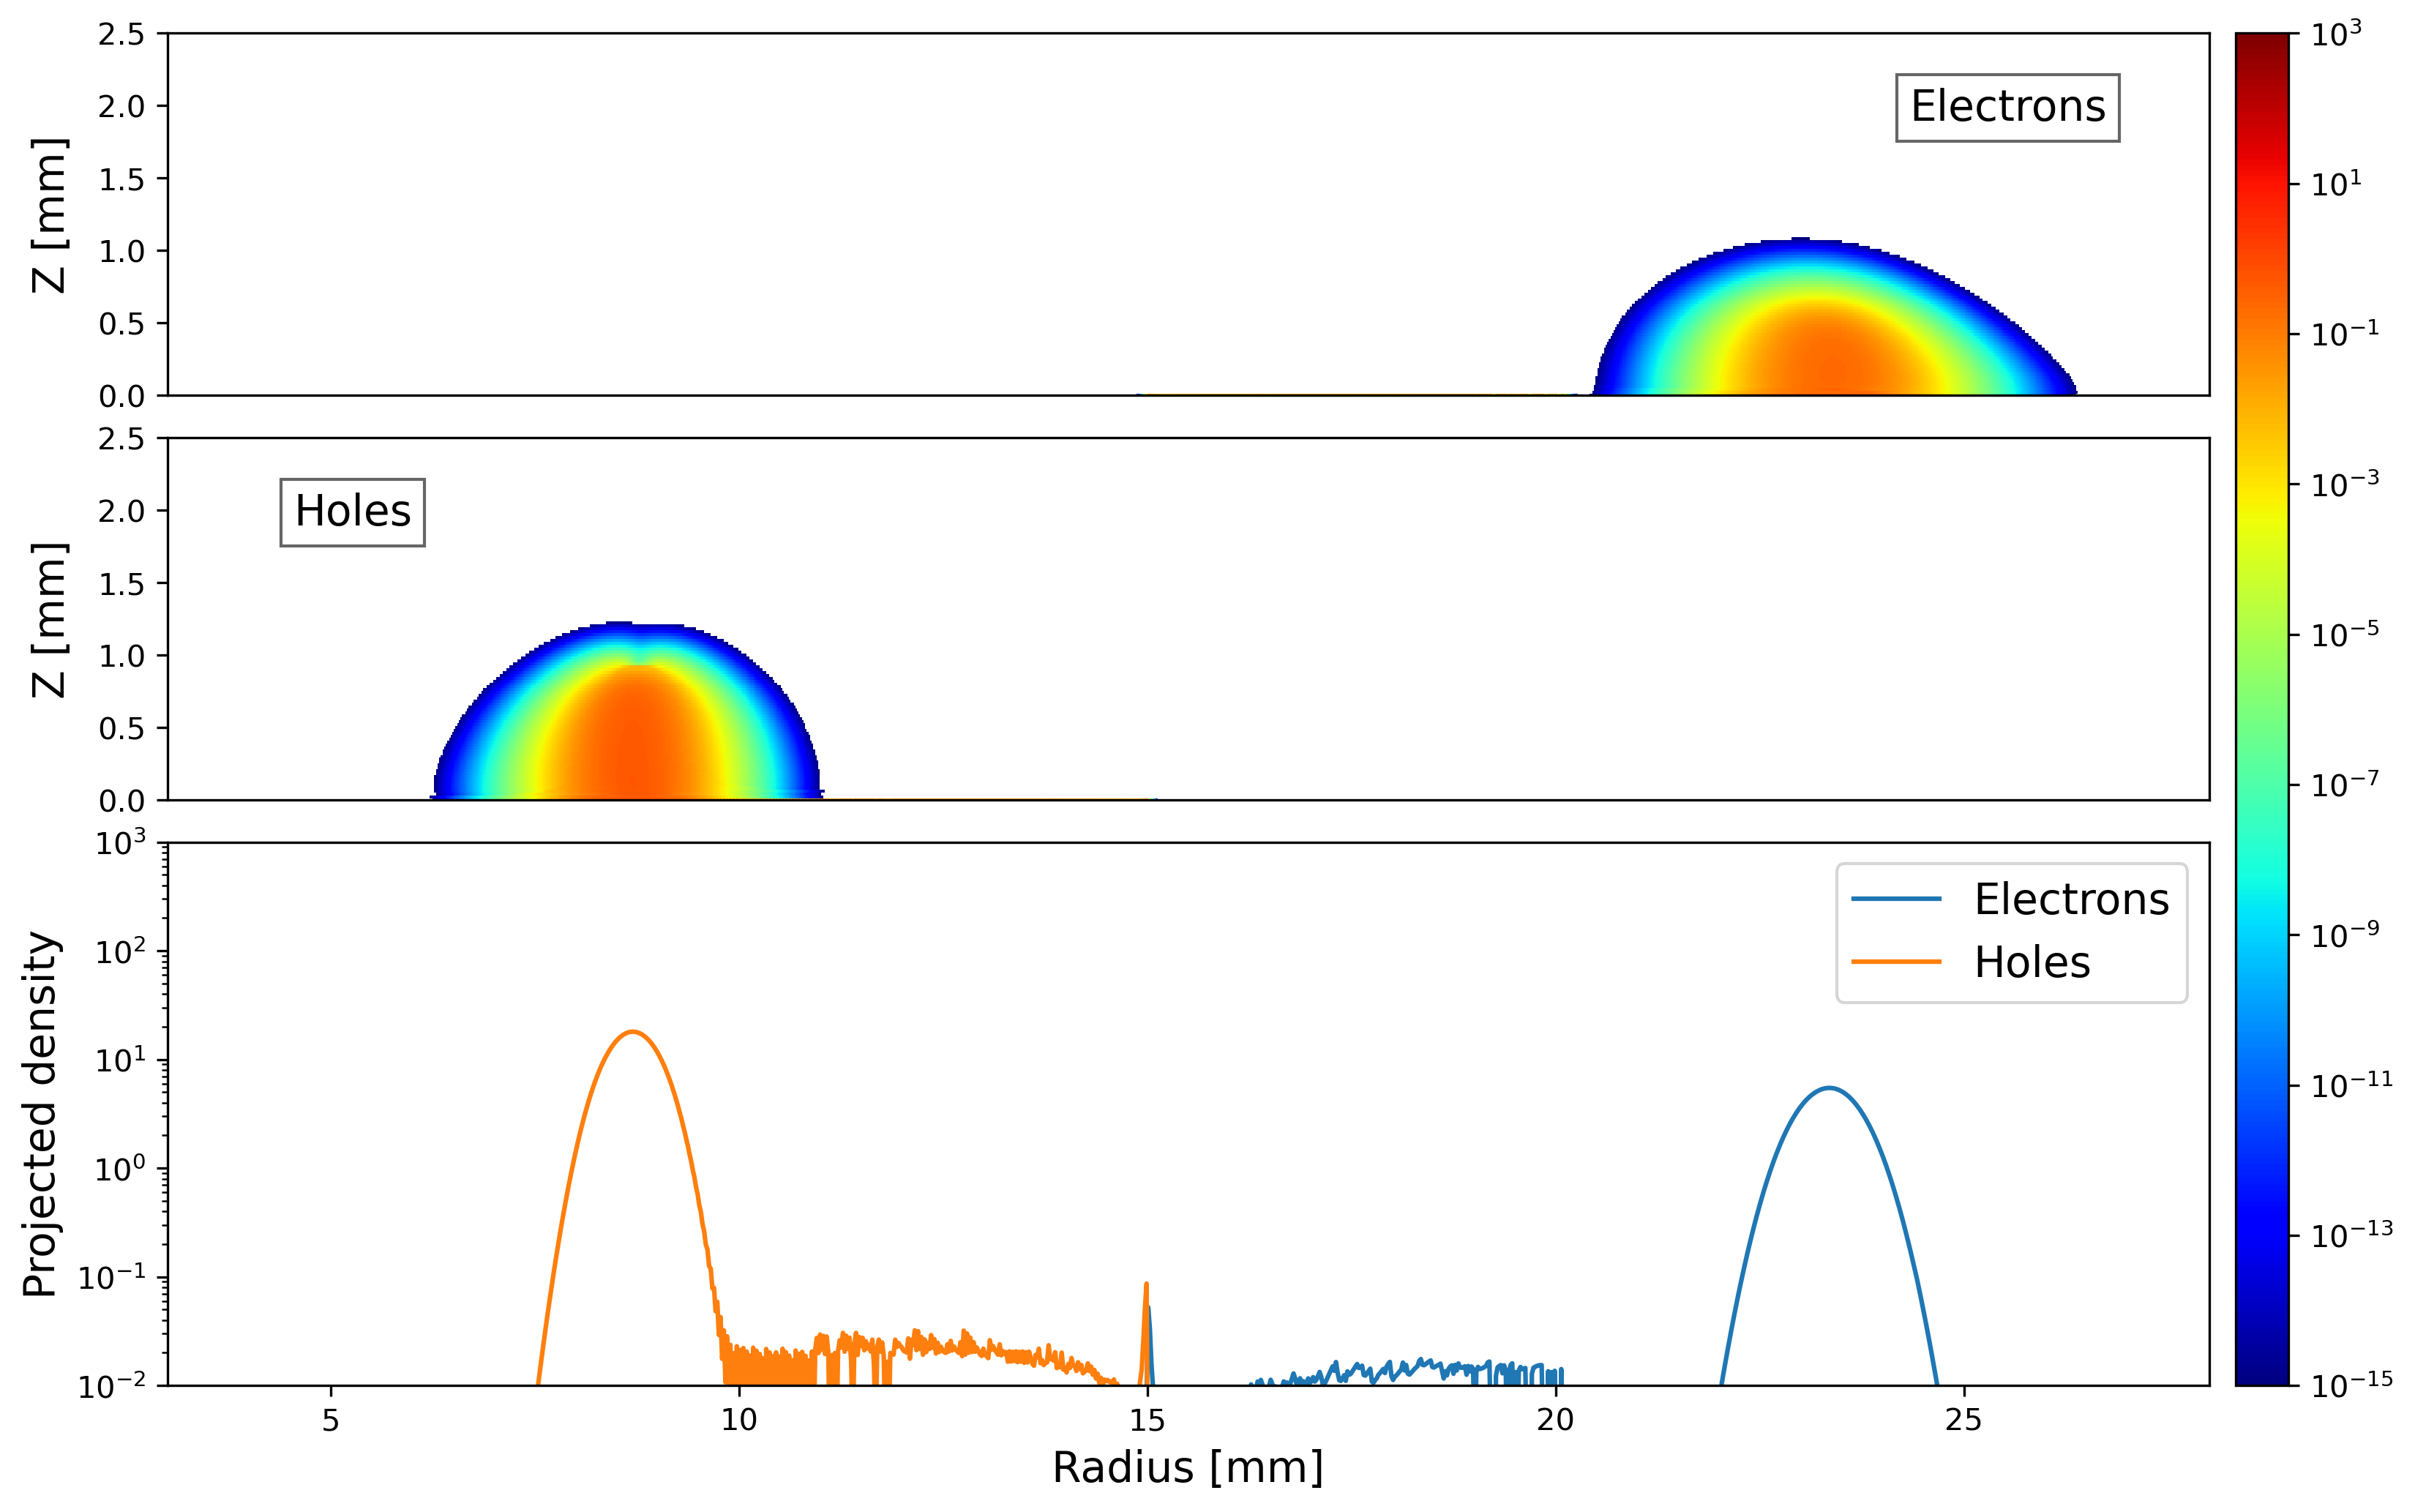
\includegraphics[trim={0cm 0 0cm 0},clip,width=0.99\linewidth]{ch3/figs/drift_path_sc=0.0.png}
    \caption{Drift of electron and hole charge clouds in {\ehd}. The projected densities show how the charges are distributed along the radius. The density have two peak, one due to fast moving component in bulk and another due to slow moving component on the passivated surface.}
    \label{ch3_fig_ehd_path_pd_sc_0}
\end{figure}

Fig. \ref{ch3_fig_ehd_path_pd_sc_neg_0p3} shows the same event but with a negative charge on the surface. The negative charges alter the field in a way that the holes are pulled onto the surface, and electrons are repelled. Thus, the holes component has significant charges attracted to the surface, as shown by their projected densities. Electrons, being repelled from the surface, have no slow-moving component.


\begin{figure}%[!htb]
    %[trim={left bottom right top},clip]
    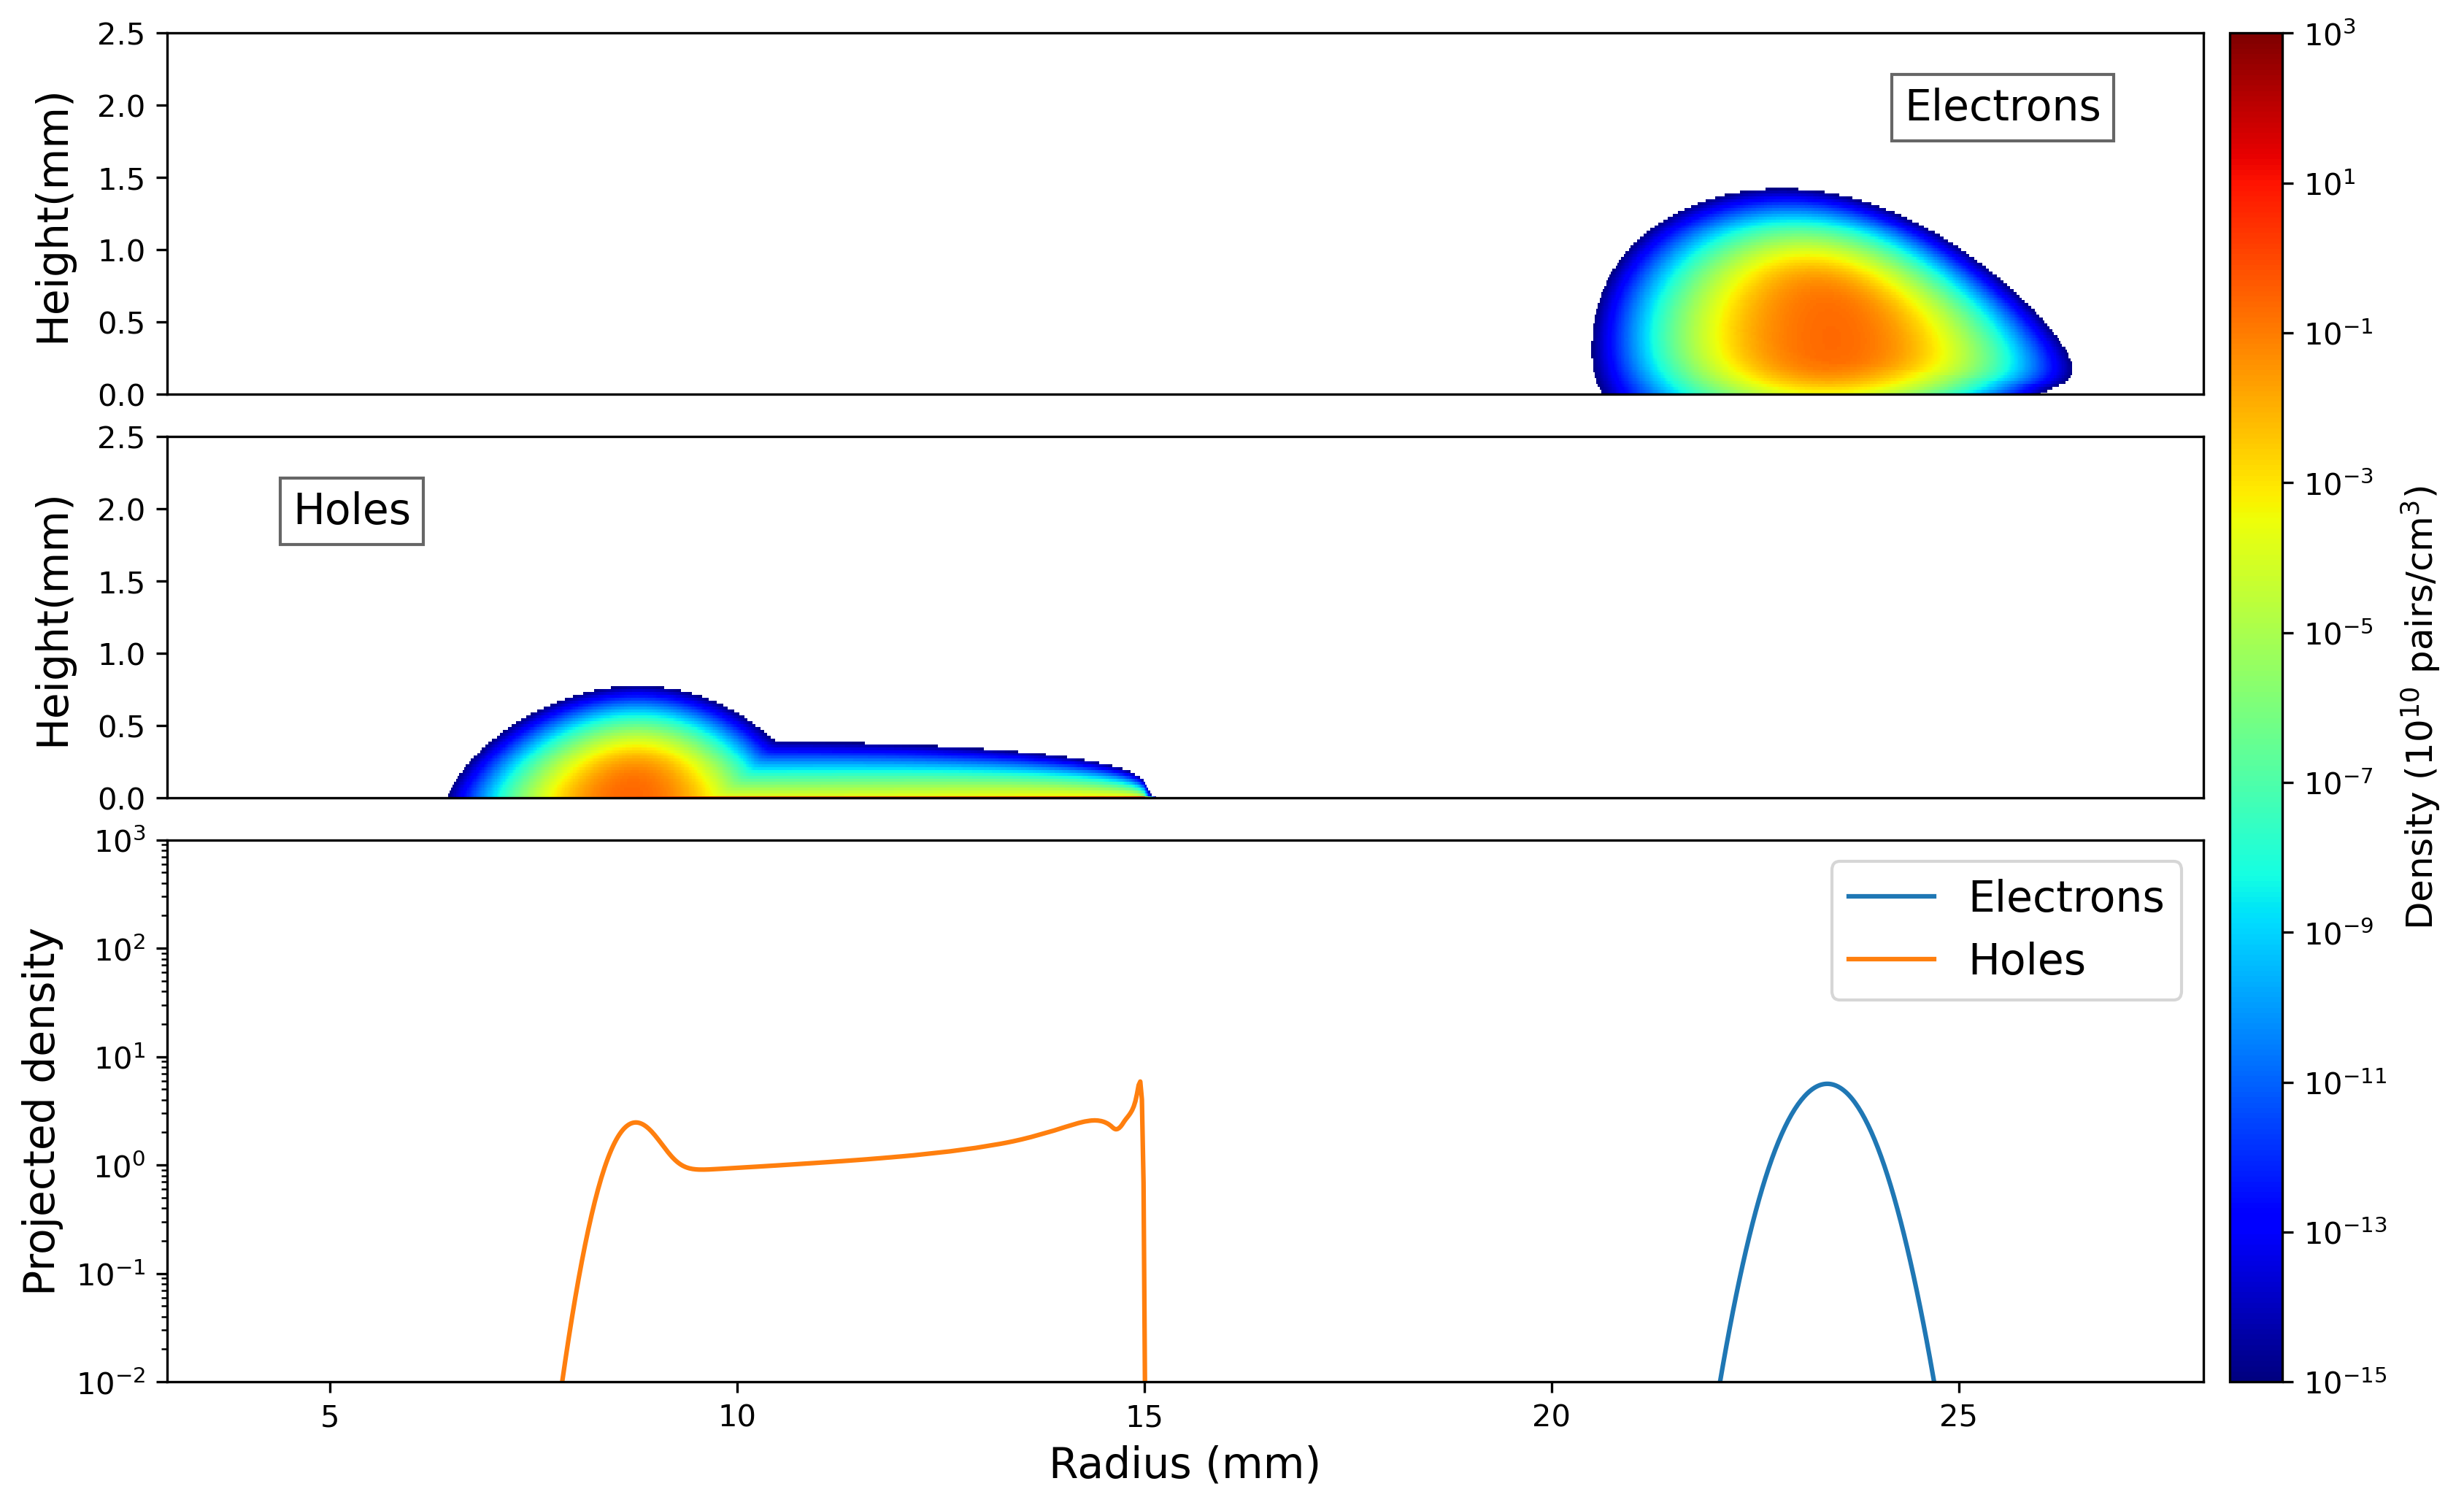
\includegraphics[trim={0cm 0 0cm 0},clip,width=0.99\linewidth]{ch3/figs/drift_path_sc=-0.3.png}
    \caption{Drift of electron and hole charge clouds in {\ehd} with negative surface charge. The negative surface charge pulls the holes onto the surface which move at a slower speed.}
    \label{ch3_fig_ehd_path_pd_sc_neg_0p3}
\end{figure}

Similarly Fig. \ref{ch3_fig_ehd_path_pd_sc_pos_0p3} shows the same event but with a positive charge on the surface. In this case, the electrons are pulled onto the surface and drift slowly, while the holes are repelled and have no surface drift. 

\begin{figure}%[!htb]
    %[trim={left bottom right top},clip]
    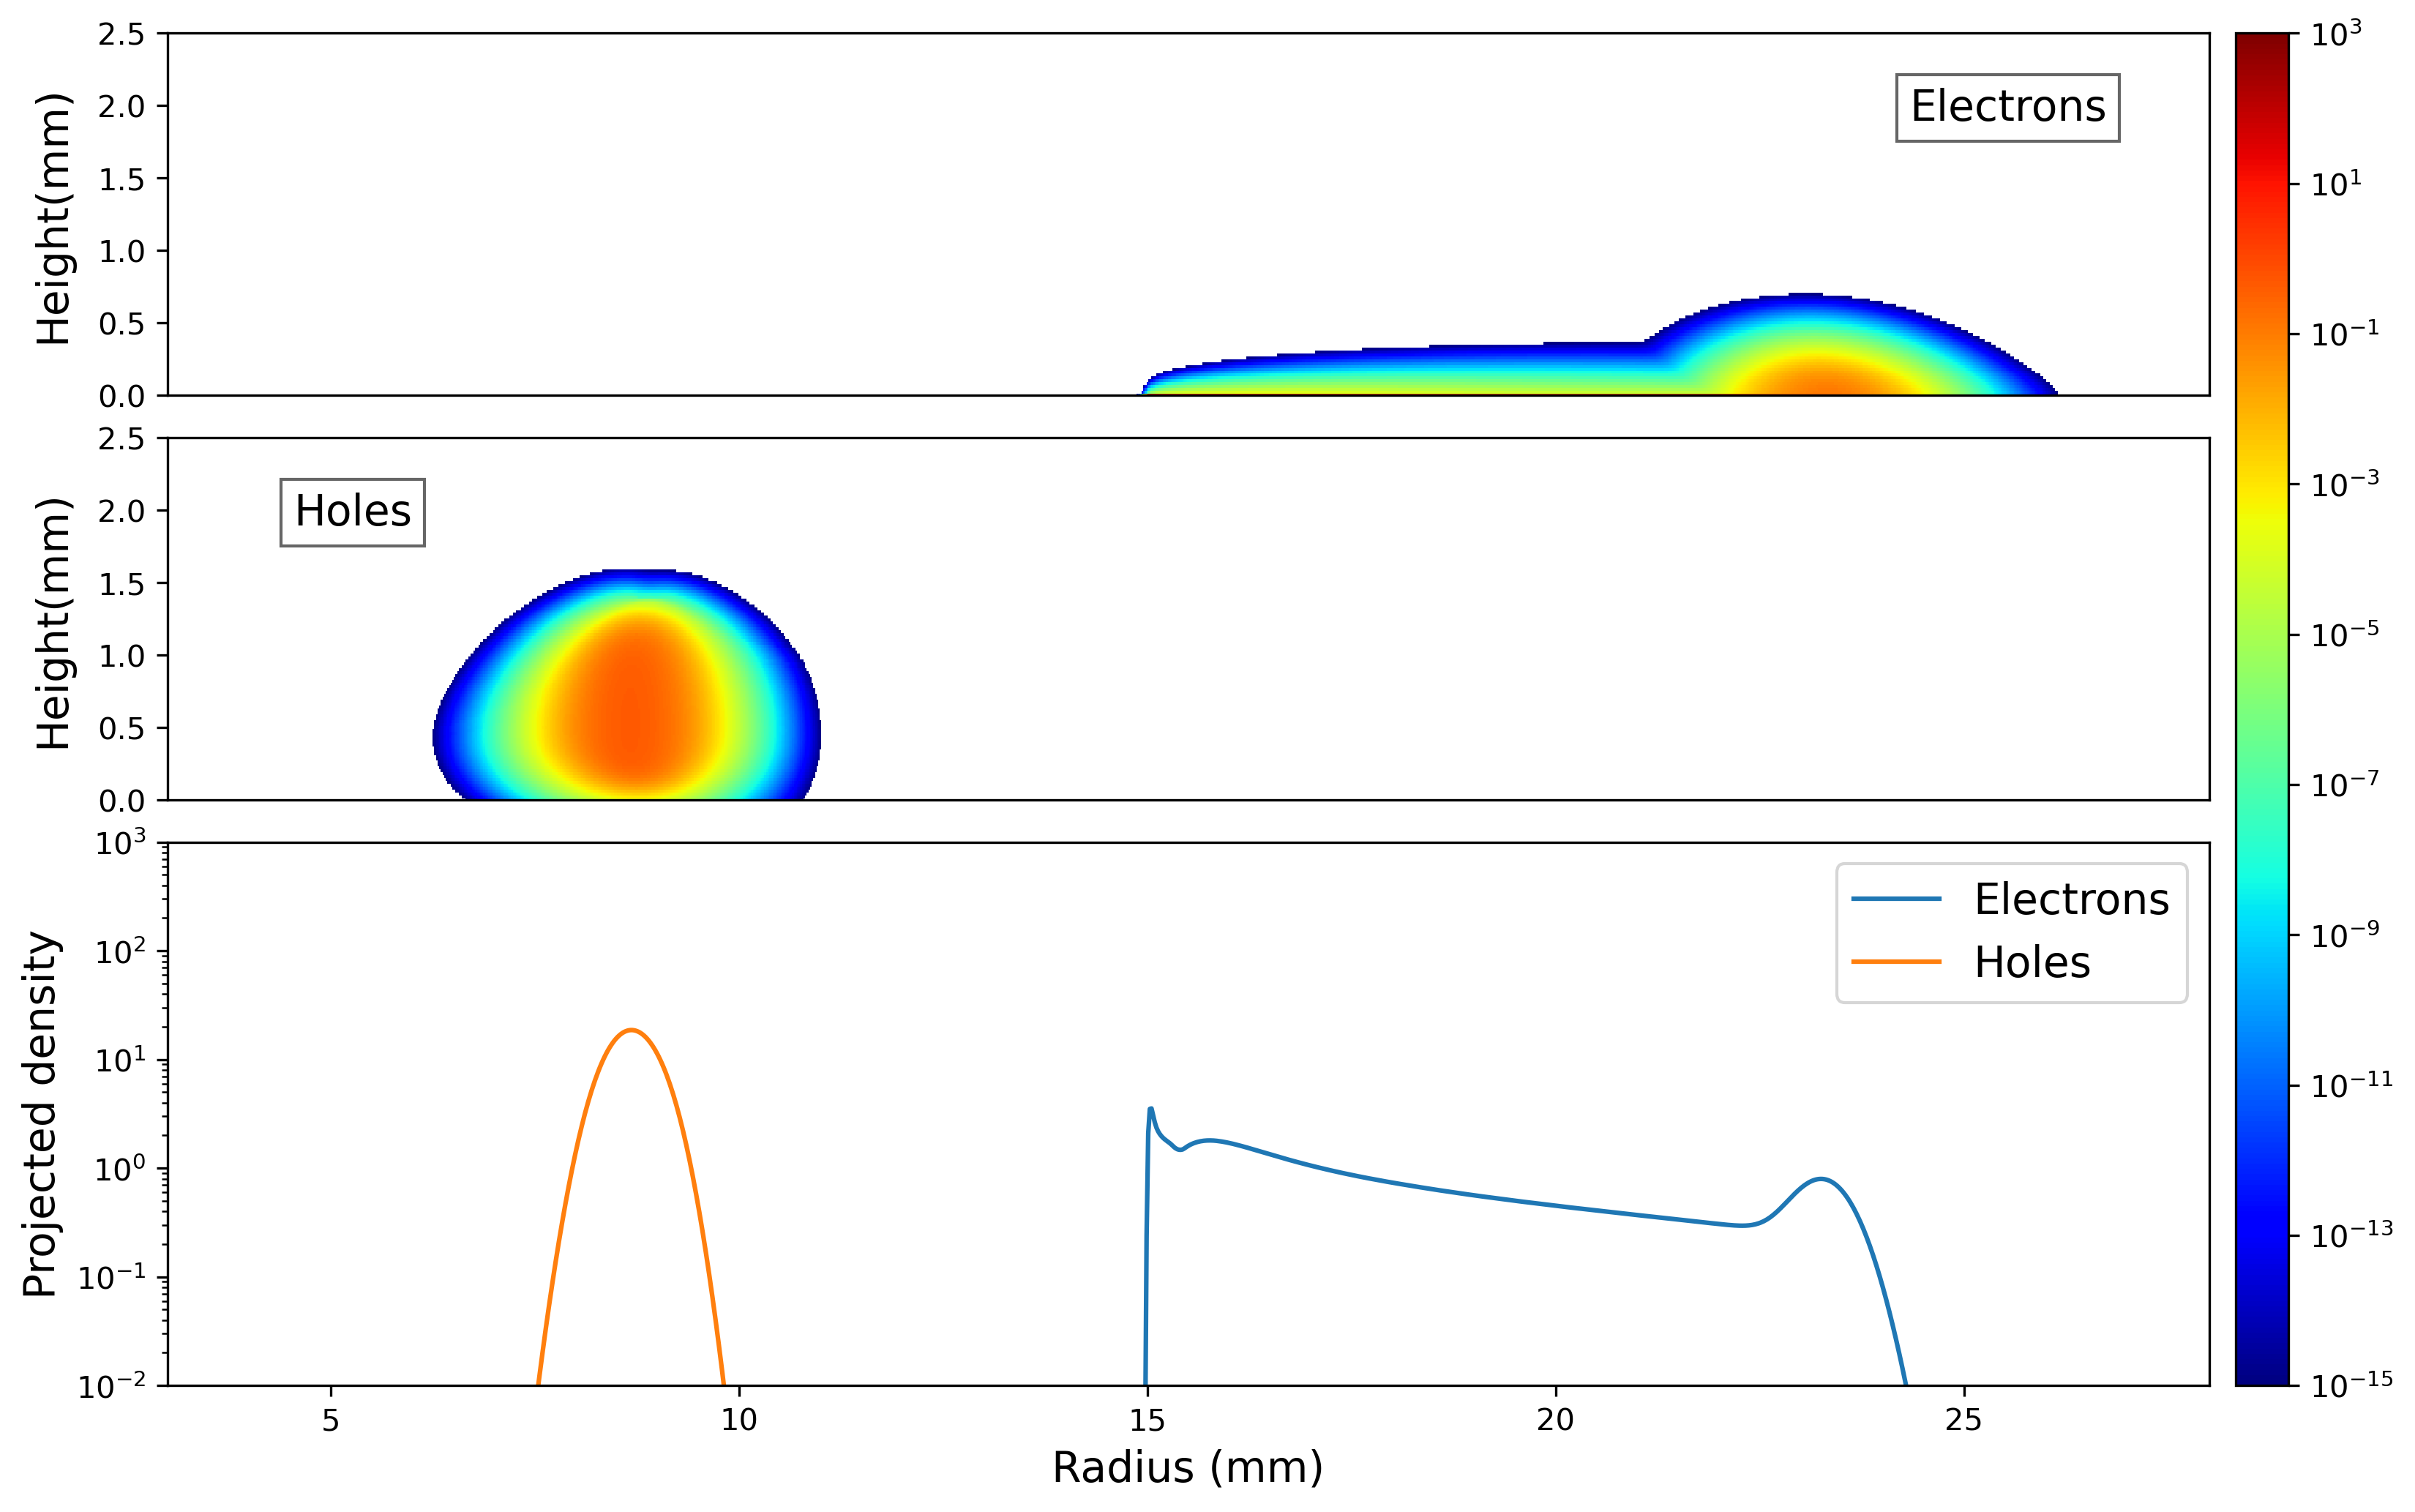
\includegraphics[trim={0cm 0 0cm 0},clip,width=0.99\linewidth]{ch3/figs/drift_path_sc=0.3.png}
    \caption{Drift of electron and hole charge clouds in {\ehd} with positive surface charge. The positive surface charge pulls the electrons onto the surface which move at a slower speed.}
    \label{ch3_fig_ehd_path_pd_sc_pos_0p3}
\end{figure}


\section{Tunable Parameters}
{\ehd} also provides several custom tunable parameters such as surface charge, surface to bulk drift ratio, initial energy, passivated surface depth, etc. that can be used to match the data. Fig. \ref{fig:wf_comp} illustrates how the output changes with surface to bulk drift and surface charge. High surface charge means that more charges will be pulled onto the surface and thus a sharp rising part will have a lower magnitude. A faster surface to bulk ratio means that the charges on the surface will be collected faster and so the tail shape will be different. Together these tunable parameters enable fine-tuning the simulations to match the observed data.

\begin{figure}%[!htb]
    %[trim={left bottom right top},clip]
    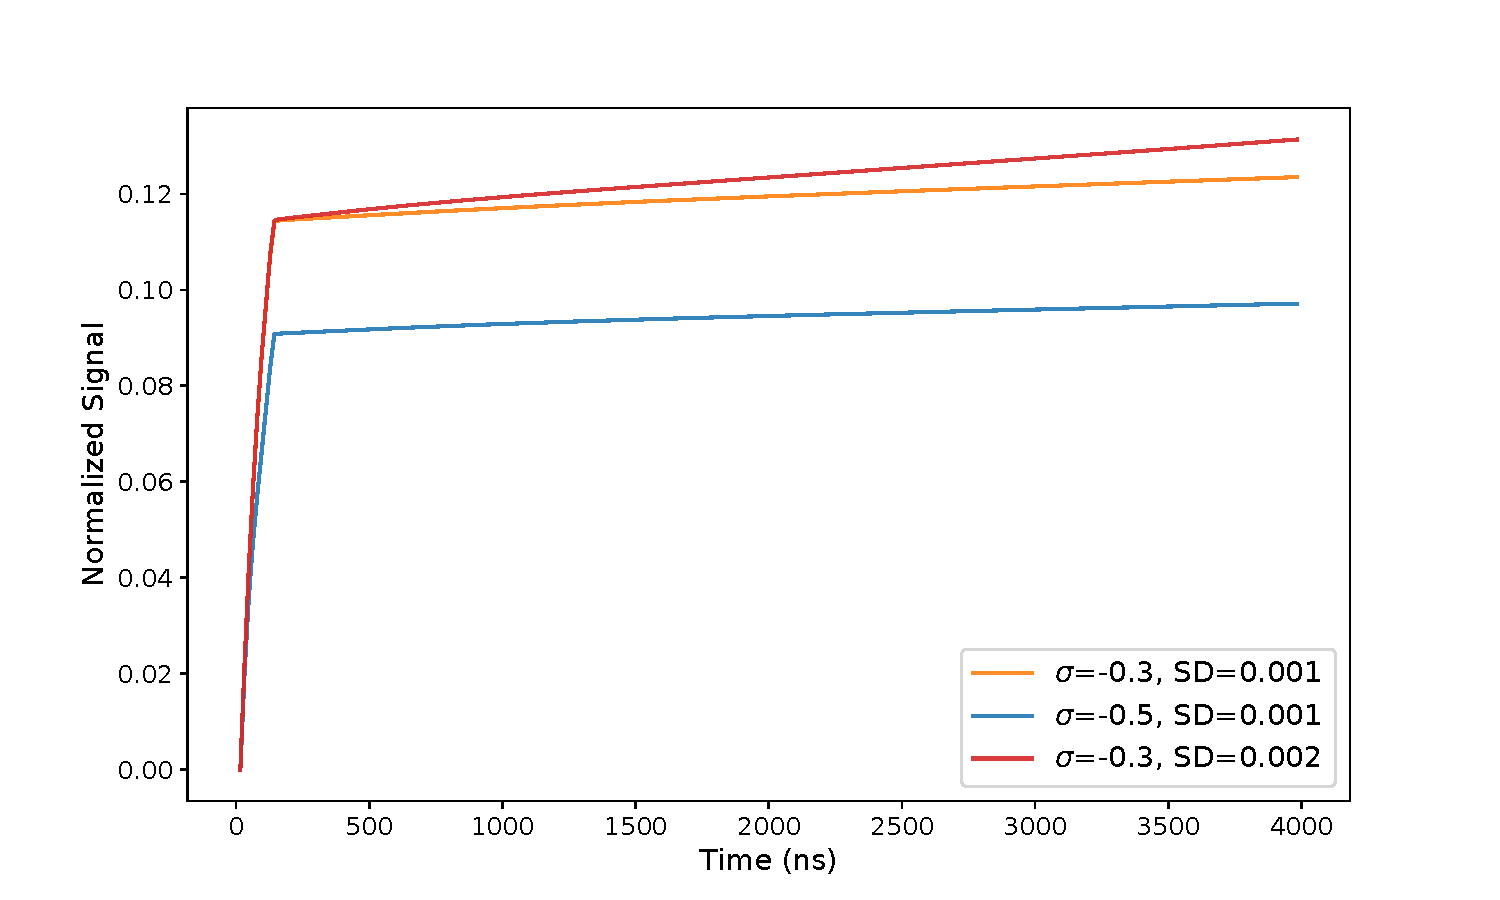
\includegraphics[trim={0.1cm 0.3cm 1.3cm 0.3cm},clip,width=0.99\linewidth]{ch3/figs/wf_comp.pdf}
    \caption{A comparison of waveforms generated by {\ehd} for a {\Ltwo} PPC detector based of different tunable parameters surface charge ($\sigma$) and relative surface drift velocity (SD).}
    \label{fig:wf_comp}
\end{figure}


\section{Input and Output}
{\ehd} is compiled using the gcc compiler. It takes in a config file same as that of {\siggen}.The config file contains information about detector geometry, and an example can be found at \cite{ehdrift2024}. In addition to the config file, we provide flags that can be passed to the executable. Table \ref{ch3_tab_ehdrift_parameters} shows the input flags that allow setting multiple parameters related to the event.
\begin{table}[!htb]
    \centering
    \renewcommand{\arraystretch}{1.3} % Adjust row spacing
    \begin{tabular}{|l|p{10cm}|c|}
        \hline
        \textbf{Flag} & \textbf{Description} & \textbf{Example} \\ 
        \hline
        -r & Set the radial position of the event in mm. & 15.00 \\
        \hline
        -z & Set the axial position of the event in mm. & 0.50 \\
        \hline
        -g & Specify the detector name. & P42575A \\
        \hline
        -s & Set the surface charge density in $10^{10} e/\text{cm}^2$. & -0.50 \\
        \hline
        -e & Input the interaction energy in keV. & 5000 \\
        \hline
        -v & Choose whether to write density files (0 = no, 1 = yes). & 1 \\
        \hline
        -f & Choose whether to recalculate the electric field (0 = no, 1 = yes). & 1 \\
        \hline
        -w & Choose whether to save the electric field (0 = no, 1 = yes). & 1 \\
        \hline
        -d & Choose whether to save the depletion surface (0 = no, 1 = yes). & 1 \\
        \hline
        -p & Choose whether to write the weighting potential (0 = no, 1 = yes). & 1 \\
        \hline
        -b & Set the bias voltage in volts. & 3500 \\
        \hline
        -h & Specify the grid size in mm. & 0.0200 \\
        \hline
        -m & Define the passivated surface depth in mm. & 0.10 \\
        \hline
        -c & Set the velocity of surface charges compared to bulk. & 0.75 \\
        \hline
        -a & Input a custom impurity density profile file. & filename.dat \\
        \hline
        -t & Define the total simulation run time in ns. & 16000 \\
        \hline
        -u & Set the frequency of output signal saving in ns. & 16 \\
        \hline
    \end{tabular}
    \caption{Input parameters to EH-Drift}
    \label{tab:ehdrift_parameters}
\end{table}



The simulation output is stored in an HDF5 file, a hierarchical data format optimized for handling large structured datasets. Each simulated event is recorded in the ``event data'' dataset as a compound data type containing energy, radius, and height positions, surface charge, surface drift velocity factor, and the signal for the event. The dataset is dynamically extendable to allow new events to be appended without rewriting existing data. The file includes grid size, passivated surface thickness, self-repulsion flag, and detector name as attributes. Attributes are stored as scalars at the file root level for efficient retrieval without redundancy. This storage is critical for High Performance Computing (HPC) when we simulate thousands of waveforms for multiple detectors.

% To summarize, surface backgrounds are an important component in the LEGEND background model, and are difficult to model. We developed a new method that can model these challenging backgrounds. In the next chapter, we discuss a method to optimize these simulations.

